\documentclass[11pt,a4paper]{article}

% ---------------------------------------------------------------------------
% Layout and fonts (house style of the leanSig / leanXMSS notes)
% ---------------------------------------------------------------------------
\usepackage[a4paper,margin=2.5cm]{geometry}
\usepackage[T1]{fontenc}
\usepackage[utf8]{inputenc}
\usepackage[final]{microtype}
\usepackage{xspace}

% ---------------------------------------------------------------------------
% Mathematics
% ---------------------------------------------------------------------------
\usepackage{amsmath}
\usepackage{amsthm}
\usepackage{mathtools}
% newpx must come after amsthm.
\usepackage{newpxtext}
\usepackage{newpxmath}

% ---------------------------------------------------------------------------
% Tables, lists, algorithms, figures
% ---------------------------------------------------------------------------
\usepackage{booktabs}
\usepackage{tabularx}
\usepackage{array}
\usepackage{multirow}
\usepackage{enumitem}
\usepackage{algorithm}
\usepackage[noend]{algpseudocode}
\usepackage{caption}
\usepackage{flafter}
\usepackage{tikz}
\usetikzlibrary{arrows.meta,decorations.pathreplacing,positioning,calc,fit}
\usepackage{xcolor}

% ---------------------------------------------------------------------------
% Links and cross-references
% ---------------------------------------------------------------------------
\definecolor{linkblue}{RGB}{0,51,153}
\definecolor{accent}{RGB}{31,94,160}
\definecolor{warn}{RGB}{176,48,32}
\usepackage[colorlinks=true,linkcolor=linkblue,citecolor=linkblue,
            urlcolor=linkblue,bookmarksnumbered=true,
            pdftitle={leanSeal: Time-Lock Encryption from Hashes Alone},
            pdfauthor={Vitalik Buterin, Quang Dao, Justin Drake}]{hyperref}
\usepackage[nameinlink,capitalise,noabbrev]{cleveref}

% ---------------------------------------------------------------------------
% Project macros
% ---------------------------------------------------------------------------
\newcommand{\leanseal}{leanSeal\xspace}
% Repository URL. Its final home is not decided yet: change it here only.
\newcommand{\repourl}{https://github.com/leanEthereum/leanSeal}
\newcommand{\repo}{\expandafter\url\expandafter{\repourl}}

% Notation for leanSeal (follows SPEC.md, Section 1).
\newcommand{\ctx}{\mathit{ctx}}
\newcommand{\salt}{\mathit{salt}}
\newcommand{\lbl}[1]{\mathsf{#1}}
\newcommand{\Hlab}[1]{\mathsf{H}_{\lbl{#1}}}
\newcommand{\Hstart}{\Hlab{start}}
\newcommand{\Hmask}{\Hlab{mask}}
\newcommand{\Hacc}{\Hlab{acc}}
\newcommand{\Hkey}{\Hlab{key}}
\newcommand{\Hcommit}{\Hlab{commit}}
\newcommand{\Henc}{\Hlab{enc}}
\newcommand{\Hmk}{\Hlab{mac}}
\newcommand{\THash}{\mathsf{TH}}
\newcommand{\SHA}{\mathsf{SHA256}}
\newcommand{\HMAC}{\mathsf{HMAC}}
\newcommand{\trunc}[2]{[#1]_{#2}}
\newcommand{\cat}{\mathbin{\|}}
\newcommand{\Build}{\mathsf{Build}}
\newcommand{\Open}{\mathsf{Open}}
\newcommand{\Qpre}{Q_{\mathrm{pre}}}
\newcommand{\Qon}{Q_{\mathrm{on}}}
\newcommand{\Qenc}{Q_{\mathrm{enc}}}
\newcommand{\Advhide}{\mathrm{Adv}^{\mathrm{hide}}}
\newcommand{\Advprf}{\mathrm{Adv}^{\mathrm{prf}}}
\newcommand{\Tkey}{T_{\mathrm{key}}}
\newcommand{\lpub}{\ell_{\mathrm{pub}}}
\newcommand{\Rs}{R_{\mathrm{s}}}
\newcommand{\Adv}{\mathcal{A}}
\newcommand{\Real}{\mathsf{R}}
\newcommand{\Ideal}{\mathsf{G}}
\newcommand{\Bad}{\mathsf{Bad}}
\newcommand{\texp}{t_{\mathrm{exp}}}
\newcommand{\torder}{t_{\mathrm{order}}}
\newcommand{\tsolve}{t_{\mathrm{solve}}}
\newcommand{\lattacker}{\ell_{\mathrm{attacker}}}
\newcommand{\lsolver}{\ell_{\mathrm{solver}}}
\newcommand{\hashlabel}[1]{\texttt{leanseal/v1/#1}}
\newcommand{\magic}[1]{\texttt{"#1"}}
% Status tags in tables (the "chips" of the web version).
\newcommand{\tagm}[1]{\textsc{#1}}


% ---------------------------------------------------------------------------
% Theorem environments
% ---------------------------------------------------------------------------
\theoremstyle{plain}
\newtheorem{theorem}{Theorem}
\newtheorem{conjecture}{Conjecture}
\newtheorem{claim}{Claim}
\theoremstyle{definition}
\newtheorem{assumption}{Assumption}
\newenvironment{claimproof}%
  {\begin{proof}[Proof of the claim]\renewcommand{\qedsymbol}{$\lozenge$}}%
  {\end{proof}}

\crefname{claim}{Claim}{Claims}
\crefname{conjecture}{Conjecture}{Conjectures}
\crefname{algorithm}{Algorithm}{Algorithms}
\crefname{ALG@line}{line}{lines}
\Crefname{ALG@line}{Line}{Lines}

% ---------------------------------------------------------------------------
% Typographic settings
% ---------------------------------------------------------------------------
\setlist{itemsep=2pt,topsep=4pt}
\captionsetup{font=small,labelfont=bf,margin=0.5cm}
\captionsetup[table]{skip=4pt}
\renewcommand{\arraystretch}{1.12}
\setcounter{tocdepth}{2}
\algrenewcommand\algorithmiccomment[1]{\hfill\(\triangleright\) {\itshape #1}}

\title{\textbf{\leanseal: Time-Lock Encryption from Hashes Alone}}
\author{%
  Vitalik Buterin\textsuperscript{1}%
  \and Quang Dao\textsuperscript{2}%
  \and Justin Drake\textsuperscript{1}}
\date{%
  \small
  \textsuperscript{1}Ethereum Foundation\\
  \texttt{vitalik@ethereum.org}, \texttt{justin.drake@ethereum.org}\\[3pt]
  \textsuperscript{2}Carnegie Mellon University\\
  \texttt{qvd@andrew.cmu.edu}\\[8pt]
  October 2026}

\begin{document}

\maketitle

\begin{abstract}
\noindent
An encrypted mempool lets block builders order transactions before they can read them. The transactions must then be opened by some party: a committee adds trust assumptions for both privacy and liveness, and a sender that opens its own transaction can withhold its key when the ordering is unfavorable. We present \leanseal, in which the sender opens its own transaction but attaches a time-lock puzzle built from SHA-256 alone, so that anyone can open the transaction without the sender after a fixed amount of sequential computation, chosen to exceed the time needed to fix the order: about 30 seconds on Ethereum. For a well-formed puzzle, withholding the key then cannot keep the transaction hidden, without a committee or a trusted setup; it can still delay or cancel the transaction's execution, which a deposit must deter.

The puzzle is the chained-hash puzzle of Mahmoody, Moran and Vadhan (CRYPTO 2011). For our encoding we prove, in the random-oracle model, that a classical attacker with the hash rate of the whole Bitcoin network derives the key early with probability at most about $2^{-117}$ for a 30-second lock. Against an attacker who computes one chained SHA-256 every 3.5\,ns, a 30-second puzzle costs the sender about 21\,s on a laptop CPU, can be built before the transaction exists, and adds 152 to 512 bytes to the transaction; opening with the revealed key takes 12\,ms. We also identify what \leanseal cannot provide: like every time lock, it also discloses transactions that are never included. We show how deposits, validity windows and composition with a committee mitigate its limitations, and compare it with threshold, TEE and hybrid designs.

\medskip
\noindent\textbf{Code, specification and benchmark logs:} \repo
\end{abstract}

\clearpage

\begingroup
\small
\tableofcontents
\endgroup
\clearpage

\section{Introduction}\label{sec:intro}

In an encrypted mempool, block builders order transactions before they can read them, which removes their ability to front-run or sandwich a transaction based on its contents. The hard question is who opens the transactions afterwards. There are three answers in current designs, and each has a cost.
\begin{itemize}[leftmargin=1.5em]
  \item \textbf{A committee} holds a threshold decryption key and opens what was ordered, as in Shutter~\cite{Shutter}. Privacy then rests on no threshold of its members colluding, and liveness on enough of them being online.
  \item \textbf{A trusted execution environment} opens transactions inside hardware whose vendor and side channels must be trusted.
  \item \textbf{The sender} opens its own transaction after the ordering, as in sealed transactions and the self-decryption path of LUCID~\cite{LUCID}. No one else is trusted, but the sender sees the ordering first and can withhold its key when the ordering does not suit it: a free option.
\end{itemize}
Hybrid designs~\cite{WM25} let either the sender or a committee open, which removes the free option while the committee is online and the committee's liveness problem while the sender is honest. Their bad case remains a dishonest sender while the committee is offline.

\leanseal makes the free option observable and penalizable without any committee. The sender opens its own transaction in the normal case, but it attaches a time-lock puzzle that anyone can solve to recover the key after a fixed amount of sequential computation, about 30 seconds on Ethereum. For a well-formed puzzle, withholding the key therefore cannot keep a transaction hidden, though it can still delay or cancel its execution; a deposit forfeited on a missed reveal must deter that. This is a timed commitment~\cite{BN00}. The puzzle uses only SHA-256: it needs no trusted setup, no committee and no hardware trust, and the idealized version is secure against quantum openers. The price is the sender's work. The puzzle is the chained-hash puzzle of Mahmoody, Moran and Vadhan~\cite{MMV11}, in which the sender computes as many hashes as an opener, only in parallel, and they proved that no hash-only puzzle can do better. This paper asks whether that price is affordable for sealing transactions, and what an encrypted mempool built on it can and cannot provide.

\begin{table}[t]
  \centering\small
  \caption{The reference puzzle at a glance: a 30-second lock of $n = 16$ chains of $2^{29}$ SHA-256 steps with 24-byte links. Times are on an Apple M4 MacBook Air (\cref{sec:costs}); building and forced opening are half our measurements of the one-minute puzzle ($m = 2^{30}$, run with 32-byte links and the same chain work), since both are linear in the delay.}
  \label{tab:glance}
  \begin{tabularx}{\textwidth}{@{}Xrl@{}}
    \toprule
    & Value & Basis \\
    \midrule
    Earliest opening by an attacker & 30\,s & \tagm{assumed}: 3.5\,ns per chained hash \\
    Opening when the sender reveals the key, the normal case & 12.0\,ms & \tagm{measured}: command line, end to end \\
    Forced opening without the sender, one laptop core & 3\,min 21\,s & \tagm{measured}, halved \\
    Building the puzzle, before the transaction exists & 21\,s & \tagm{measured}, halved: all CPU cores \\
    Added to a transaction, on-demand or stockpiled puzzle & 512 or 152\,B & exact \\
    \bottomrule
  \end{tabularx}
\end{table}

\paragraph{Our results.}
\begin{enumerate}[label=\arabic*.,leftmargin=1.5em]
  \item \textbf{A design.} We describe \leanseal as a decryption path for an encrypted mempool: self-decryption with a time-lock fallback (\cref{sec:mempool}). It uses the same data as LUCID and the hybrid design, a ciphertext bound to a commitment to its key, so its puzzle fits them as a fallback that needs no third party.
  \item \textbf{A concrete security proof.} In the random-oracle model, a classical attacker derives the key even one oracle round early with probability at most about $2^{-117}$ for a 30-second lock against the hash rate of the whole Bitcoin network (\cref{sec:security}). Turning rounds into seconds needs one hardware number, the fastest time for one chained SHA-256, which we price at 3.5\,ns, 3.7 times faster than the fastest published design we found.
  \item \textbf{Affordable costs.} A 30-second puzzle, enough when the order is fixed within a slot, takes about 21\,s to build on a laptop CPU and can be built before the transaction exists (\cref{sec:choosing-t} chooses the delay per use case). A sender that keeps a stock can use single-chain puzzles, which add 152 bytes to a transaction (\cref{sec:costs}).
  \item \textbf{An honest account of the trade-offs.} A time lock also reveals transactions that are never included; we argue that this holds for every design whose fallback opening is input-free, and show how validity windows, private submission and a committee limit it. Withholding can still delay or cancel execution, so a deposit carries the economics; the reveal deadline makes a missed reveal observable, and the time lock separately ensures that a well-formed puzzle is eventually disclosed (\cref{sec:tradeoffs}). We compare \leanseal with threshold, TEE, hybrid and delay-encryption designs (\cref{sec:comparison}).
  \item \textbf{An implementation}: a specified format with a Rust implementation, a second implementation in Python, test vectors and benchmarks, and a prototype on an EVM chain that demonstrates sealed submission, key revelation, ordered execution within a batch and forced disclosure; its searcher sandwiches only plaintext swaps, for a 9.25\% loss, so it does not yet demonstrate sandwich protection (\cref{sec:poc})~\cite{leanSealRepo}.
\end{enumerate}
Neither the puzzle nor its implementation is new in itself (\cref{sec:related}). What is new is a concrete bound for an exact encoding, measured costs against an explicit attacker, and its analysis as an encrypted mempool.

\section{Sealing Transactions with \leanseal}\label{sec:mempool}

This section treats the puzzle as a black box and describes how it backs an encrypted mempool. The sender runs $\Build$ to get a puzzle $Z$, which contains a commitment $C$, and a key $K$. Anyone can check a claimed key against $C$ with one hash. Anyone can also recover $K$ from $Z$ alone with $N$ sequential hashes, which takes at least $T = N\ell$ seconds on the fastest hardware. \Cref{sec:construction,sec:security} construct the puzzle and prove this.

\subsection{The flow}\label{sec:flow}

\leanseal is used as a timed commitment~\cite{BN00}; \cref{fig:commit-reveal} shows the flow.
\begin{enumerate}[leftmargin=1.5em]
  \item \textbf{Submit.} The sender takes a puzzle from its stock and encrypts its signed transaction under $K$. It sends the sealed transaction together with a plaintext envelope: the account that pays, a nonce, a gas limit, a fee and a deposit (\cref{sec:admission}).
  \item \textbf{Order.} The builder orders sealed transactions without reading them. The ordering commits to the hash of each whole sealed transaction, not just to $C$: once $K$ is known, anyone could seal a different transaction under the same puzzle.
  \item \textbf{Reveal.} Once the ordering is fixed, the sender publishes $K$. Nodes check it against $C$, decrypt in about 12\,ms and execute the transaction in its committed position. Nobody solves anything.
  \item \textbf{Fallback.} If the sender stays silent past the reveal deadline, its deposit is forfeited, and anyone can solve the puzzle and publish $K$. A well-formed puzzle therefore opens without its sender, but its transaction can only run late or not at all.
\end{enumerate}

% Commit-reveal with a time-lock fallback (Figure 3 of the web version).
\begin{figure}[t]
  \centering
  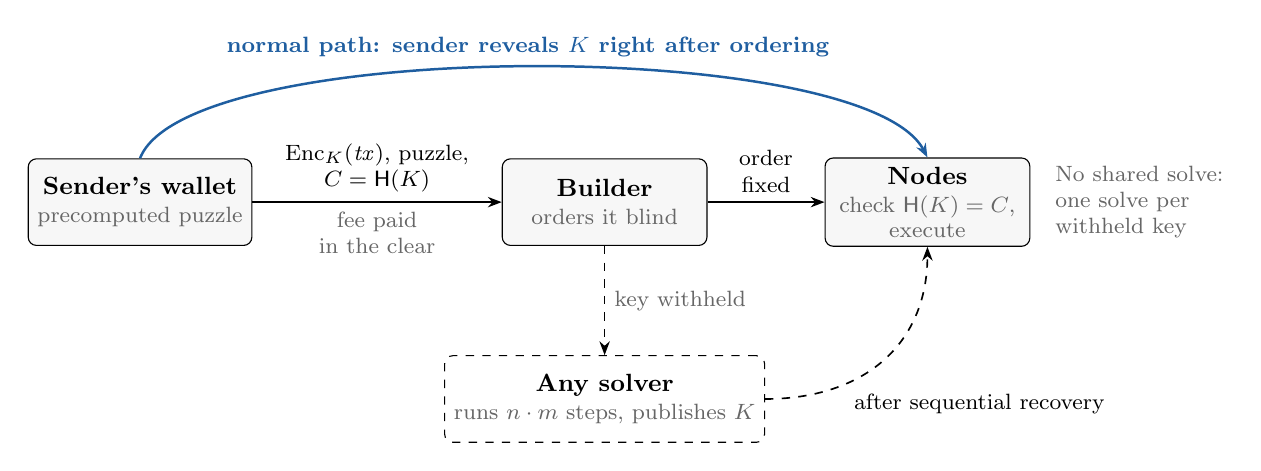
\begin{tikzpicture}[
      x=1cm, y=1cm, font=\small,
      box/.style={draw, rounded corners=3pt, minimum height=1.1cm, align=center, fill=black!3},
      sub/.style={font=\footnotesize, text=black!60},
      lab/.style={font=\footnotesize, align=center},
      arr/.style={-{Stealth[length=5pt]}, line width=0.6pt},
    ]
    \node[box, minimum width=2.8cm] (wallet) at (1.4,0)
      {\textbf{Sender's wallet}\\[-1pt]{\footnotesize\color{black!60}precomputed puzzle}};
    \node[box, minimum width=2.6cm] (builder) at (7.3,0)
      {\textbf{Builder}\\[-1pt]{\footnotesize\color{black!60}orders it blind}};
    \node[box, minimum width=2.6cm] (nodes) at (11.4,0)
      {\textbf{Nodes}\\[-1pt]{\footnotesize\color{black!60}check $\mathsf{H}(K) = C$,}\\[-2pt]{\footnotesize\color{black!60}execute}};
    \node[box, dashed, fill=none, minimum width=3.6cm] (solver) at (7.3,-2.5)
      {\textbf{Any solver}\\[-1pt]{\footnotesize\color{black!60}runs $n \cdot m$ steps, publishes $K$}};
    % Main path.
    \draw[arr] (wallet) -- node[lab, above] {$\mathrm{Enc}_K(\mathit{tx})$, puzzle,\\$C = \mathsf{H}(K)$}
                          node[lab, below, text=black!60] {fee paid\\in the clear} (builder);
    \draw[arr] (builder) -- node[lab, above] {order\\fixed} (nodes);
    % Normal path: the user reveals K.
    \draw[arr, accent, line width=0.9pt]
      (wallet.north) .. controls (2.0,2.1) and (10.6,2.1) .. (nodes.north)
      node[pos=0.5, above, font=\footnotesize\bfseries, text=accent] {normal path: sender reveals $K$ right after ordering};
    % Fallback: the user stays silent.
    \draw[arr, dashed] (builder.south) -- node[lab, right, text=black!60] {key withheld} (solver.north);
    \draw[arr, dashed] (solver.east) .. controls (10.6,-2.5) and (11.4,-1.8) .. (nodes.south)
      node[pos=0.3, below right, lab] {after sequential recovery};
    % Side note.
    \node[sub, align=left, anchor=west] at (12.9,0) {No shared solve:\\one solve per\\withheld key};
  \end{tikzpicture}
  \caption{Commit--reveal with a time-lock fallback. When senders reveal their keys, no puzzle is solved. For a well-formed puzzle, withholding the key cannot prevent disclosure, but it can still delay or cancel execution.}
  \label{fig:commit-reveal}
\end{figure}


A ciphertext bound to a commitment to its key is the shape that recent Ethereum designs already use. In LUCID (EIP-8184)~\cite{LUCID}, a sealed transaction's ticket goes on chain and carries a commitment $\mathsf{keccak256}(k_{\mathrm{dem}})$ to the key and a hash of the ciphertext envelope, which itself travels off chain. The key is released by a key publisher of the sender's choice, possibly the sender itself, and the publication fee is paid only when decryption succeeds. In the hybrid design of Wagner and Ma~\cite{WM25}, the sender puts $\mathrm{Enc}_k(\mathit{tx})$ and $\mathsf{H}(k)$ on chain and gives a committee a threshold encryption of $k$, so that either the sender or the committee can open. \leanseal fits both as a fallback that needs no third party: the sender is its own key publisher, and the puzzle replaces the committee as the party that discloses the key when the sender does not. Inside LUCID only the puzzle is used. It travels in the envelope's opaque header with $K$ as $k_{\mathrm{dem}}$; its SHA-256 commitment $C$ is separate from the ticket's keccak commitment, and the cipher stays ChaCha20-Poly1305. The puzzle provides eventual disclosure only: executing a transaction whose key is disclosed minutes late needs an additional protocol rule, which LUCID does not have.

The reveal should be due as soon as the ordering is fixed. In LUCID, the builder's bid commits to the tickets of slot $n$, keys are released once the payload is out and must be seen before the payload-timeliness committee votes, and the decrypted transactions execute at the top of block $n+1$, before any ordinary transaction. A short window shortens the delay the puzzle must provide and limits what a sender learns before deciding whether to reveal (\cref{sec:withholding}).

\subsection{The timing condition}\label{sec:timing}

The attacker's clock starts at \emph{exposure}, $\texp$, the first moment anyone but the sender holds the puzzle. The deadline $\torder$ is the moment the transaction's position can no longer change. The contents stay hidden until the deadline if
\[
  \torder - \texp < N \cdot \lattacker,
\]
with a margin for propagation. A forced opening finishes $N \cdot \lsolver$ after a solver starts, which on a laptop core is minutes after the deadline. If the attacker is $k$ times faster than assumed, the delay shrinks $k$-fold; once it falls below $\torder - \texp$, the contents can be read before the order is fixed. Privacy before ordering is then lost and content-dependent MEV becomes possible again, for whoever can solve fast enough.

\subsection{Choosing the delay}\label{sec:choosing-t}

The delay should be the smallest that covers the time from exposure to the fixed order, $\torder - \texp$. Building, forced opening, the solvers' load and the window in which a silent sender holds an option all grow linearly with $T$; only the size does not. The attacker speed already carries a margin of about 3.7 over the fastest published design (\cref{sec:pricing}), so we take $T$ about twice the time to fix the order. \Cref{tab:choosing-t} applies this to the settings of \cref{sec:realistic}. We use $T = 30$\,s as the reference: it covers a puzzle that is sent only to the slot's builder, or published after a commitment, and ordered within one 12-second slot.

\begin{table}[t]
  \centering\small
  \caption{The delay per setting. Building uses all cores of the M4 Air (0.70\,s per second of delay); forced opening uses one of its cores (6.6 times the delay).}
  \label{tab:choosing-t}
  \begin{tabularx}{\textwidth}{@{}>{\raggedright\arraybackslash}X>{\raggedright\arraybackslash}p{2.7cm}rrr@{}}
    \toprule
    Setting & Time to fix the order & Delay $T$ & Building & Forced opening \\
    \midrule
    Rollup with a sequencer & 1--2\,s & 15\,s & 11\,s & 1.7\,min \\
    Ethereum with enshrined PBS; puzzle sent to the builder, or published after a commitment & up to one slot, 12\,s & \textbf{30\,s} & 21\,s & 3.3\,min \\
    Sealed-bid auction; bid committed, then posted near the close & about one slot & 30\,s & 21\,s & 3.3\,min \\
    Public gossip, waiting $w$ slots & $12(w+1)$\,s & $24(w+1)$\,s & $17(w+1)$\,s & $2.7(w+1)$\,min \\
    Order fixed only at finality, Ethereum today & about 13\,min & 15\,min & 10.5\,min & 1.7\,h \\
    \bottomrule
  \end{tabularx}
\end{table}

The last row is why \leanseal needs an order that is fixed early. Waiting for today's finality makes every cost thirty times larger than in the reference setting, so a protocol either accepts that a reorganization exposes revealed transactions (\cref{sec:reorgs}) or relies on fast finality, which brings the delay back to the reference range. Public gossip is affordable for a wait of a slot or two but not more, which is why the puzzle should not wait in a public mempool.

\subsection{What \leanseal provides}\label{sec:mempool-props}

\Cref{tab:props} lists the properties an encrypted mempool may want and what \leanseal gives. No known design gives all of them; \cref{sec:comparison} compares the alternatives.

\begin{table}[t]
  \centering\small
  \caption{Properties of an encrypted mempool, and what \leanseal provides.}
  \label{tab:props}
  \begin{tabularx}{\textwidth}{@{}>{\raggedright\arraybackslash}p{4.3cm}>{\raggedright\arraybackslash}X@{}}
    \toprule
    Property & \leanseal \\
    \midrule
    Contents hidden until the order is fixed & yes, for $T$ after exposure, under the hardware assumption \\
    Every included transaction opens & yes, without the sender or anyone else, if the puzzle is well formed \\
    No free cancellation after seeing the order & no: withholding still delays or, with expiry, cancels execution; a deposit must deter it (\cref{sec:withholding}) \\
    Excluded transactions stay private & no: they open after $T$ like any other (\cref{sec:noninclusion}) \\
    Sender, fee and size hidden & no; the envelope is public and the size can be padded \\
    Trusted parties or setup & none \\
    Post-quantum & plausibly; proved for the idealized puzzle only (\cref{sec:attacks}) \\
    Cost & 152 to 512 bytes per transaction, sender work proportional to $T$ paid in advance, no work for the network in the normal case (\cref{sec:costs}) \\
    \bottomrule
  \end{tabularx}
\end{table}

\subsection{A proof of concept}\label{sec:poc}

We implemented this flow as a contract on any chain with EIP-7702, with off-chain sender, keeper and solver roles~\cite{leanSealRepo}. The block that includes a sealed transaction fixes its position within its batch. The sender reveals its key within two blocks, and anyone then executes the batch's revealed transactions in order: the contract checks each key against its commitment and decrypts the envelope, both with SHA-256 only, and calls the sender's account, which delegates to the contract for this. A missed reveal lets anyone who later finds the key from the puzzle open the transaction. On a local chain with 2-second blocks, a searcher watching the mempool sandwiched a plaintext swap, which lost 9.25\% against the fair price; the same swap, sealed, executed at the fair price. With its key withheld, a demonstration puzzle of $2^{29}$ steps, 1/16 of the reference work, was solved on one core in 19.5\,s and the swap executed late.

The prototype demonstrates submission, key revelation, ordered execution within a batch and forced disclosure. It does not demonstrate sandwich protection. Its searcher attacks only plaintext submissions. Once a key is revealed, anyone can decrypt the transaction and trade against the same pool before the separate execution call, and batches from different blocks can execute out of order. A deployment must reserve the execution position relative to every transaction that touches the same state, as LUCID does by executing decrypted transactions at the top of the next block; fixing the block that contains the submission is not enough. Nor does the prototype implement the deterrent: the deposit of a missed reveal goes to whoever posts the key, and the withholding sender knows it, so it can recover its own deposit. A deployment must separate an irrecoverable penalty from any solver reward. In the contract's unit tests, with a 128-byte test puzzle, submitting costs about 199{,}000 gas and revealing about 74{,}000, and a batch of two swaps executes for about 155{,}000 gas per swap including decryption. These are contract-call costs; calldata and intrinsic costs come on top and grow with the envelope.

\section{The Puzzle}\label{sec:construction}

A \emph{hash chain} starts from a value and hashes it many times in a row. Each step needs the previous output, so even unlimited hardware needs the steps one after another. A single chain of $N$ steps would make a fine lock, except that its builder also needs $N$ sequential steps. The construction of Mahmoody, Moran and Vadhan~\cite{MMV11} fixes this: the sender builds $n$ short chains of $m$ steps at the same time and links them so that an opener can only run them in order. The opener's delay is $N = nm$ steps; the sender's wall time is $m$ steps on $n$ cores.

\subsection{Notation and model}\label{sec:prelims}\label{sec:notation}

The notation follows the specification (\texttt{SPEC.md} in the repository~\cite{leanSealRepo}). Integers are encoded big-endian, $a \cat b$ is concatenation, $\trunc{v}{b}$ is the first $b$ bytes of $v$, and $\oplus$ is bytewise XOR. A \emph{labelled hash} is $\THash(\mathit{label}, x) = \SHA(\mathsf{u8}(|\mathit{label}|) \cat \mathit{label} \cat x)$, and we write $\Hstart, \Hmask, \Hacc, \Hkey, \Hcommit$ for labelled hashes with the labels \hashlabel{start}, \hashlabel{mask} and so on. The \emph{chain step} for chain $i$ is
\[
  F_i(s) = \SHA\bigl(s \cat \salt \cat \mathsf{be32}(i)\bigr),
\]
where $\salt$ is 16 random bytes drawn for each puzzle. Its input is exactly 52 bytes, so one step is one SHA-256 compression, and no other hash in the format has an input of that length. A puzzle has $n$ chains of $m$ steps and $b$-byte links. The reference parameters are $n = 16$, $m = 2^{29}$ and $b = 24$: $N = 2^{33}$ steps, a 30-second delay at 3.5\,ns per step, and a 452-byte puzzle; we measured the one-minute puzzle with $m = 2^{30}$.

\label{sec:rom}We prove the delay in the random-oracle model~\cite{MMV11}: each chain step and each labelled hash is an independent random function that anyone can query, and an attacker is charged only for its queries. Time after publication is counted in \emph{oracle rounds}: all queries in a round are chosen before any answer from that round arrives. A bound in rounds therefore holds however much parallel hardware the attacker has; turning rounds into seconds takes the hardware assumption of \cref{sec:security}.

\subsection{Building and opening}\label{sec:algorithms}

\Cref{alg:build,alg:open} give the two algorithms, following Sections~4 and~5 of the specification with the byte encodings left out. The context $\ctx$ is a 32-byte encoding of the version, $b$, $n$, $m$ and the salt, and every hash other than the chain step includes it.

\begin{algorithm}[t]
  \caption{$\Build(n, m, b)$, run by the sender}\label{alg:build}
  \begin{algorithmic}[1]
    \State $\salt \gets$ 16 random bytes; \ $x_1, \dots, x_n \gets$ $b$ random bytes each
    \State $\ctx \gets (1, b, n, m, \salt)$
    \For{$i = 1, \dots, n$ \textbf{in parallel}}\label{line:build-for}
      \State $s_i \gets \Hstart(\ctx, i, x_i)$
      \State $y_i \gets F_i^m(s_i)$ \Comment{$m$ sequential steps}\label{line:build-chain}
    \EndFor
    \For{$i = 1, \dots, n - 1$}
      \State $z_i \gets \trunc{\Hmask(\ctx, y_i)}{b} \oplus x_{i+1}$ \Comment{hide the next link}\label{line:build-mask}
    \EndFor
    \State $a \gets \ctx$\label{line:build-acc}
    \State \algorithmicfor\ $i = 1, \dots, n$ \algorithmicdo\ $a \gets \Hacc(a, y_i)$
    \State $K \gets \Hkey(\ctx, a)$; \ $C \gets \Hcommit(\ctx, K)$\label{line:build-key}
    \State \Return puzzle $Z = (\ctx, C, x_1, z_1, \dots, z_{n-1})$ and key $K$
  \end{algorithmic}
\end{algorithm}

\begin{algorithm}[t]
  \caption{$\Open(Z)$, run by anyone}\label{alg:open}
  \begin{algorithmic}[1]
    \State parse $Z$ as $(\ctx, C, x_1, z_1, \dots, z_{n-1})$
    \State $x \gets x_1$; \ $a \gets \ctx$
    \For{$i = 1, \dots, n$} \Comment{in sequence}
      \State $y \gets F_i^m(\Hstart(\ctx, i, x))$ \Comment{$m$ sequential steps}
      \State $a \gets \Hacc(a, y)$ \Comment{lines~\ref{line:open-acc} and~\ref{line:open-mask} share one oracle round}\label{line:open-acc}
      \State \algorithmicif\ $i < n$ \algorithmicthen\ $x \gets \trunc{\Hmask(\ctx, y)}{b} \oplus z_i$ \Comment{unhide $x_{i+1}$}\label{line:open-mask}
    \EndFor
    \State $K \gets \Hkey(\ctx, a)$
    \State \algorithmicif\ $\Hcommit(\ctx, K) \neq C$ \algorithmicthen\ \Return $\bot$ \Comment{malformed puzzle}\label{line:open-check}
    \State \Return $K$
  \end{algorithmic}
\end{algorithm}

The sender knows every link, so it runs the $n$ chains of \cref{alg:build} in parallel. Each link after the first is published only masked, under a hash of the end of the chain before it. The key is a hash of all chain ends in order, and the commitment $C$ lets anyone check a claimed key with one hash. An opener without the key has only $x_1$: it runs chain~1, uses its end to unhide $x_2$, runs chain~2, and so on, $nm$ steps in sequence (\cref{fig:schedules}). The only way to start a chain early is to guess its link. The sender encrypts the transaction under $K$ with HMAC-SHA256 (\cref{sec:costs}) and keeps the puzzle and key until it needs them.

% Parallel building versus sequential opening (Figure 2 of the web version).
\begin{figure}[t]
  \centering
  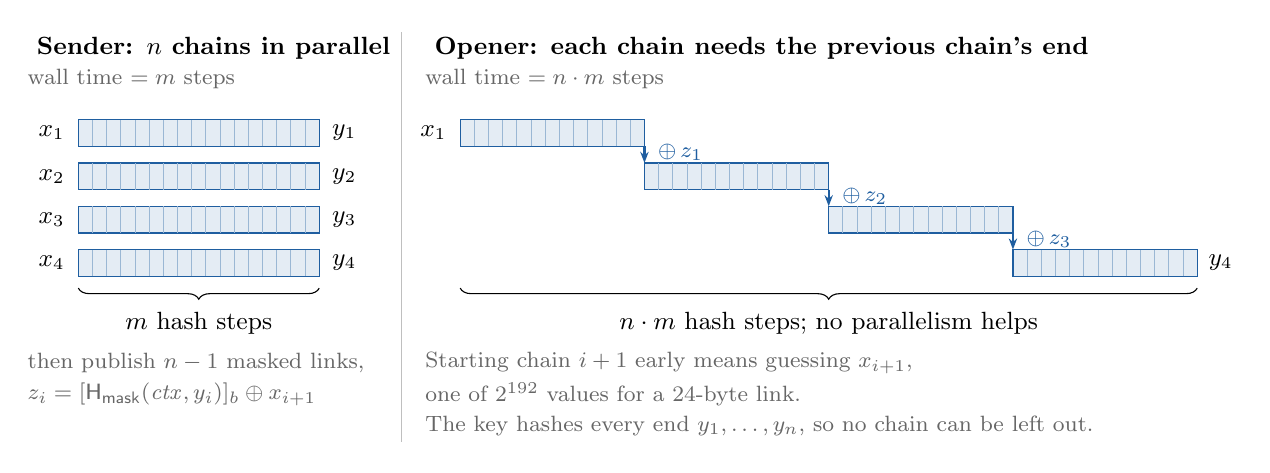
\begin{tikzpicture}[
      x=1cm, y=1cm, font=\small,
      chain/.style={draw=accent, fill=accent!12, line width=0.5pt},
      note/.style={font=\footnotesize, text=black!60, align=left, anchor=west, inner xsep=0pt},
      head/.style={font=\small\bfseries, anchor=west},
    ]
    % Bar of m steps, with tick marks for the individual steps.
    \newcommand{\chainbar}[3]{% x0, y, width
      \draw[chain] (#1,#2) rectangle ++(#3,0.34);
      \foreach \t in {0.18,0.36,...,#3} {
        \draw[accent!45, line width=0.3pt] ({#1+\t},#2) -- ++(0,0.34);
      }
    }
    % ---------------- Sender ----------------
    \node[head] at (-0.3,1.25) {Sender: $n$ chains in parallel};
    \node[note] at (-0.3,0.85) {wall time $= m$ steps};
    \foreach \i/\y in {1/0, 2/-0.55, 3/-1.10, 4/-1.65} {
      \chainbar{0.35}{\y}{3.06}
      \node[anchor=east] at (0.3,\y+0.17) {$x_{\i}$};
      \node[anchor=west] at (3.45,\y+0.17) {$y_{\i}$};
    }
    \draw[decorate, decoration={brace, mirror, amplitude=4pt}]
      (0.35,-1.80) -- node[below=5pt] {$m$ hash steps} (3.41,-1.80);
    \node[note] at (-0.3,-2.75) {then publish $n - 1$ masked links,};
    \node[note] at (-0.3,-3.15) {$z_i = \trunc{\Hmask(\ctx, y_i)}{b} \oplus x_{i+1}$};
    % ---------------- Divider ----------------
    \draw[black!25] (4.45,1.45) -- (4.45,-3.75);
    % ---------------- Opener ----------------
    \node[head] at (4.75,1.25) {Opener: each chain needs the previous chain's end};
    \node[note] at (4.75,0.85) {wall time $= n \cdot m$ steps};
    \foreach \i/\x/\y in {1/5.20/0, 2/7.54/-0.55, 3/9.88/-1.10, 4/12.22/-1.65} {
      \chainbar{\x}{\y}{2.34}
    }
    \node[anchor=east] at (5.15,0.17) {$x_1$};
    \node[anchor=west] at (14.58,-1.48) {$y_4$};
    \foreach \i/\x/\y in {1/7.54/0, 2/9.88/-0.55, 3/12.22/-1.10} {
      \draw[-{Stealth[length=4pt]}, accent, line width=0.8pt] (\x,\y) -- (\x,\y-0.21);
      \node[anchor=west, text=accent, font=\footnotesize] at (\x+0.05,\y-0.08) {$\oplus\, z_{\i}$};
    }
    \draw[decorate, decoration={brace, mirror, amplitude=4pt}]
      (5.20,-1.80) -- node[below=5pt] {$n \cdot m$ hash steps; no parallelism helps} (14.56,-1.80);
    \node[note] at (4.75,-2.75) {Starting chain $i + 1$ early means guessing $x_{i+1}$,};
    \node[note] at (4.75,-3.15) {one of $2^{192}$ values for a 24-byte link.};
    \node[note] at (4.75,-3.55) {The key hashes every end $y_1, \dots, y_n$, so no chain can be left out.};
  \end{tikzpicture}
  \caption{The same $n$ chains, arranged two ways in time (drawn for $n = 4$). The sender knows every link and runs the chains side by side. An opener must run them one after another, because each chain's starting link is hidden under the end of the previous chain. The puzzle consists of the $n$ links, so its size grows with $n$ and not with the delay.}
  \label{fig:schedules}
\end{figure}


Four choices in the encoding matter for security. Every hash names its puzzle and chain, so work on another puzzle does not help. Masks are hashes of chain ends, not the ends themselves, so learning a link says nothing about the chain before it. The key depends on every chain's end, so a guessed link cannot be confirmed until the opener's own chains reach it. And the puzzle consists of $68 + nb$ bytes whatever the delay: the delay depends only on $N$.

\section{Security}\label{sec:security}

Secrecy until the deadline rests on two assumptions about SHA-256 and two about the attacker's hardware. This section states them, proves the delay in the random-oracle model, and estimates the one hardware parameter that the proof cannot supply.

\subsection{Assumptions}\label{sec:assumptions}

\begin{description}[leftmargin=1.5em,font=\normalfont\bfseries]
  \item[A1. No shortcut.] The chain step and each labelled hash behave like independent random oracles on their whole inputs. We instantiate them heuristically with SHA-256; a chain step is a single compression. If this fails, the delay is lost and the hash must be replaced, which the versioned format allows.
  \item[A2. Speed.] During the delay, no party computes one chain step in less than $\ell$. An error here shrinks the delay in proportion.
  \item[A3. Budget.] The attacker computes at most $R$ hashes per second in total. An error here multiplies the bound of \cref{thm:delay} by the same factor; for the reference puzzle, any factor up to $2^{52}$ keeps it below $2^{-64}$.
  \item[A4. Encryption.] HMAC-SHA256 is a pseudorandom function (\cref{def:prf}).
\end{description}

\subsection{The delay theorem}\label{sec:theorem}

\paragraph{Model.}
The chain steps $F_1, \dots, F_n$ and the labelled hashes of \cref{alg:build,alg:open} are independent random oracles (\cref{sec:rom}). The attacker is a classical randomized algorithm $\Adv = (\Adv_0, \Adv_1)$ with unbounded computation. $\Adv_0$ runs before the puzzle exists and makes $\Qpre$ queries; its whole state passes to $\Adv_1$, which receives the puzzle and makes $\Qon$ queries. Let $Q = \Qpre + \Qon$. Time after publication is counted in oracle rounds: all queries in a round are chosen before any answer from that round arrives.

\paragraph{Honest schedule.}
Computing each chain's mask and accumulator in the same round, $\Open$ derives $K$ in oracle round
\[
  \Tkey = n(m + 2) + 1
\]
and returns it, checked against $C$, one round later. $\Build$ takes $m + n + 3$ rounds: one for the starts, $m$ for the chains, $n$ for the accumulator, with the masks alongside, and one each for $K$ and $C$. Let $P = n(m + 3) + 1$, the number of oracle answers $\Open$ uses, $C$ included.

\begin{theorem}[Classical attackers, random-oracle model]\label{thm:delay}
Let $(Z, K) \gets \Build(n, m, b)$, with randomness independent of the oracles. For every attacker $\Adv = (\Adv_0, \Adv_1)$ as above,
\[
  \Pr\bigl[\Adv_1 \text{ outputs } K \text{ within fewer than } \Tkey \text{ oracle rounds}\bigr]
  \;\le\; \frac{\Qon}{2^{8b}} + \frac{\Qpre}{2^{128 + 8b}} + \frac{QP + P^2 + 1}{2^{256}},
\]
and the first term is absent when $n = 1$.
\end{theorem}

\paragraph{The bound in seconds.}
Assumptions A2 and A3 turn oracle rounds and queries into time. Write $T = n m \ell$, and let the attacker make $\Qon = R \cdot T$ queries after publication. Against $R = 10^{21}$ queries per second, about the hash rate of the whole Bitcoin network (\cref{sec:pricing}), the bound is about $2^{-117}$ for a 30-second lock and $2^{-97}$ for a one-year lock. Precomputation changes this only slightly: a full year of queries at the same rate before a 30-second puzzle is published adds about $2^{-128}$. With 24-byte links the first term, the chance of guessing a link, dominates; for a 30-second lock the full-width terms are smaller by a factor of about $2^{31}$. At a fixed delay the bound depends on the number of chains only weakly, through $P \approx N$, except that the first term is absent when $n = 1$. The bound covers every speed-up, however small: except with this probability, the attacker does not derive the key even one oracle round before the honest opener.

\paragraph{Scope.}
The threshold is the round in which $K$ is derived, not the round in which $\Open$ returns: an attacker that skips the check against $C$ finishes one round before $\Open$ does, with certainty. The precomputation term is needed even when $n = 1$, where the only link is public: an attacker that guesses the salt and the link in advance and computes the key opens the puzzle in zero rounds with probability $2^{-(128 + 8b)}$. The theorem concerns recovery of the key; \cref{thm:hiding} below extends it to the contents. The bounds are classical; extending them to this instantiation against quantum attackers is outside the scope of this paper.


\Cref{app:proof} gives the proof. It follows the structure of Pietrzak and Reyzin's soundness proof for proofs of sequential work~\cite{PR26}.

\paragraph{Hiding the contents.}
An attacker in an encrypted mempool also sees the envelopes sealed under $K$, and may only need to tell two candidate transactions apart. The labelled hashes $\Henc$ and $\Hmk$ that derive an envelope's subkeys are random oracles like the others, but HMAC is computed outside the oracles. This theorem, unlike \cref{thm:delay}, therefore needs the attacker's other computation to be bounded, since an unbounded attacker could evaluate HMAC under every key. We let $\Adv$ make at most $\Qpre$ and $\Qon$ oracle queries, as before, and at most $t$ further computation steps.

\begin{figure}[t]
\centering\small
\newcommand{\gamebox}[2]{\fbox{\begin{minipage}[t][3.1cm][t]{#1}#2\end{minipage}}}
\gamebox{0.27\textwidth}{$\underline{\mathsf{Hide}_\beta(\Adv)}$
\begin{algorithmic}[1]
  \State $\sigma \gets \Adv_0^{H}$
  \State $(Z, K) \gets \Build(n, m, b)$
  \State $i \gets 0$
  \State $\beta' \gets \Adv_1^{H, \mathsf{Enc}}(\sigma, Z)$
  \State \Return $\beta'$
\end{algorithmic}}\hfill
\gamebox{0.33\textwidth}{$\underline{\mathsf{Enc}(M_0, M_1)}$
\begin{algorithmic}[1]
  \State \algorithmicif\ $i = \Qenc$ \algorithmicthen\ \Return $\bot$
  \State \algorithmicif\ $|M_0| \neq |M_1|$ \algorithmicthen\ \Return $\bot$
  \State $i \gets i + 1$
  \State $\eta \gets$ 16 random bytes
  \State \Return $\mathsf{Seal}(K, \eta, M_\beta)$
\end{algorithmic}}\hfill
\gamebox{0.31\textwidth}{$\underline{\mathsf{PRF}_\beta(\mathcal{B})}$
\begin{algorithmic}[1]
  \For{$j = 1, \dots, u$}
    \State $k_j \gets$ 32 random bytes
    \State $g_j \gets \HMAC(k_j, \cdot)$
    \State \algorithmicif\ $\beta = 0$ \algorithmicthen\ $g_j \xleftarrow{\$} \mathcal{F}$
  \EndFor
  \State \Return $\mathcal{B}^{g_1, \dots, g_u}$
\end{algorithmic}}
\caption{The games of \cref{def:hiding,def:prf}. $H$ denotes all the oracles, and $\mathsf{Seal}(K, \eta, M)$ is the envelope of $M$ under $K$ with nonce $\eta$ (\cref{sec:costs}). $\mathcal{F}$ is the set of functions from byte strings to 32-byte values, and $\xleftarrow{\$}$ samples uniformly.}
\label{fig:games}
\end{figure}

\begin{definition}[Encryption game]\label{def:hiding}
For $\beta \in \{0, 1\}$, the game $\mathsf{Hide}_\beta$ and its envelope oracle $\mathsf{Enc}$ are given in \cref{fig:games}. $\Adv_0$ makes at most $\Qpre$ oracle queries; $\Adv_1$ makes at most $\Qon$ and stops within fewer than $\Tkey$ oracle rounds. The advantage of $\Adv$ is
\[
  \Advhide(\Adv) = \bigl|\Pr[\mathsf{Hide}_1(\Adv) = 1] - \Pr[\mathsf{Hide}_0(\Adv) = 1]\bigr|.
\]
\end{definition}

\begin{definition}[Pseudorandomness of HMAC]\label{def:prf}
For $\beta \in \{0, 1\}$ and $u$ keys, the game $\mathsf{PRF}_\beta$ is given in \cref{fig:games}. The advantage of an algorithm $\mathcal{B}$ is
\[
  \Advprf_u(\mathcal{B}) = \bigl|\Pr[\mathsf{PRF}_1(\mathcal{B}) = 1] - \Pr[\mathsf{PRF}_0(\mathcal{B}) = 1]\bigr|,
\]
and $\Advprf_u(t')$ is the largest advantage of an algorithm running in time $t'$.
\end{definition}

\begin{theorem}[Hiding]\label{thm:hiding}
For every attacker as above,
\[
  \Advhide(\Adv)
  \;\le\; 2\Bigl(\frac{\Qon}{2^{8b}} + \frac{\Qpre}{2^{128 + 8b}} + \frac{QP' + P'^2}{2^{256}} + \frac{\Qenc^2}{2^{129}} + \Advprf_{2\Qenc}\bigl(t + O(Q + P')\bigr)\Bigr),
\]
where $P' = P + 2\Qenc$, and the first term is absent when $n = 1$.
\end{theorem}

The first three terms come from \cref{thm:delay}, with $P'$ path values in place of $P$: each envelope adds two subkeys derived from $K$. The fourth is the chance that two nonces repeat, and the last is the cost of replacing HMAC under the $2\Qenc$ subkeys by random functions. For the reference puzzle and few envelopes, the doubled link-guessing term is about $2^{-116}$; the nonce term can dominate when many envelopes share a puzzle. The theorem says nothing from round $\Tkey$ on, when the key can be derived and every envelope under it opens. \Cref{app:hiding} gives the proof.

\subsection{The hardware assumption}\label{sec:pricing}

The attacker's total hash rate can be estimated from deployed hardware: the Bitcoin network computes about $10^{21}$ hashes per second (October 2026), and we take $R = 10^{21}$. A query is one compression, while a Bitcoin hash costs two, since it hashes twice and the first block of the header is computed once; counted in compressions, the network makes about $2 \cdot 10^{21}$ queries per second, which costs one bit: $2^{-116}$ instead of $2^{-117}$ for a 30-second lock. Mining hardware computes many independent hashes at once, of block headers rather than salted chains, and says little about how fast one hash can follow another, so it bounds $R$, not $\ell$.

The speed $\ell$ is the assumption that most needs hardware evidence. \Cref{tab:pricing} collects what is known. Relative to the fastest published design that we know of, a synthesized 7\,nm core at 13.0\,ns per hash~\cite{BCF+20}, we assume an \emph{advantage} of $A \approx 3.7$, that is, $\ell = 3.5$\,ns: 6.6 times faster than one core of the M4 laptop we measured. Some advantage over the published core is certain, since it is a general-purpose design that registers every round and does not exploit the constant part of a chain step's input; \cref{app:hardware} gives a circuit model for a chip built for chains. We do not claim 3.5\,ns is a lower bound. The theorem holds for any value of $\ell$ the reader adopts, and every cost in \cref{sec:costs} scales linearly with $1/\ell$.

\begin{table}[t]
  \centering\small
  \caption{Time per chained SHA-256 hash, from measurements to models.}
  \label{tab:pricing}
  \begin{tabularx}{\textwidth}{@{}>{\raggedright\arraybackslash}p{4.6cm}r>{\raggedright\arraybackslash}X@{}}
    \toprule
    \colhead{Source} & \colhead{Time per hash} & \colhead{Basis} \\
    \midrule
    Apple M4, one core & 23.2\,ns & \tagm{measured}: \leanseal benchmark \\
    AMD EPYC 9554P (Zen 4), one core & 37.4\,ns & \tagm{measured}: \leanseal benchmark, SHA-NI \\
    Published SHA-256 core, 7\,nm~\cite{BCF+20} & 13.0\,ns & \tagm{synthesis}: 67 cycles at 5.15\,GHz; not a fabricated chip \\
    Custom round circuit, 3--5\,nm & 2.9--9.7\,ns & \tagm{model}: \cref{app:hardware}; no such chip has been built \\
    \midrule
    \textbf{Assumed attacker} & \textbf{3.5\,ns} & the design point of this paper ($A \approx 3.7$) \\
    \bottomrule
  \end{tabularx}
\end{table}

\paragraph{Sensitivity.}
Only A1 fails abruptly. An attacker $k$ times faster than assumed opens a 30-second puzzle in $30/k$ seconds; restoring the margin costs $k$ times more sender work and no extra bytes. An attacker with $k$ times the budget multiplies the bound by $k$, which for the reference puzzle stays below $2^{-64}$ unless $k$ exceeds $2^{52}$. Slower honest hardware costs time, never secrecy. For the reference setting the margin is a factor of about 2.5: a 30-second puzzle covers a 12-second window only while one step takes more than $12\,\mathrm{s}/2^{33} \approx 1.4$\,ns. At 1.3\,ns, the advantage $A = 10$ that \cref{app:hardware} does not rule out, it opens in 11.2\,s, before the deadline. The bound of \cref{thm:delay} is negligible next to this; the hardware estimate is what limits the reference parameters. The secrecy is also temporary: a sealed transaction becomes public in any case, so only hardware that exists during its delay matters, and $\ell$ can be repriced as hardware improves.

\subsection{Attacks and link width}\label{sec:attacks}

\begin{itemize}[leftmargin=1.5em]
  \item \textbf{Link guessing.} An attacker can guess a hidden link $x_k$ and run chains $k, k+1, \dots$ while its own earlier chains are still running. This is the first term of the theorem; with 24-byte links each guess is right with probability $2^{-192}$. Because the key needs every chain's end, a guess cannot be checked against $C$ until the attacker's own chains reach link $k$.
  \item \textbf{Precomputation.} Every hash on the honest path depends on the puzzle's fresh salt and a fresh link, so work done before publication or on another puzzle does not help, except as counted by the theorem's second and third terms.
  \item \textbf{Quantum attackers.} Afshar et al.~\cite{ACHLM23} prove that the idealized chained puzzle keeps its delay against quantum openers in the quantum random-oracle model. Carrying this over to \leanseal's exact encoding has not been done; our bound is classical.
  \item \textbf{Early access.} The attacker's clock starts when it first holds the puzzle. Puzzles built in advance must stay private until use.
  \item \textbf{Message substitution.} A claimed key is checked against $C$ with one hash and the tag then authenticates the transaction. But once $K$ is known, anyone can seal a different transaction under the same puzzle, so an ordering must bind the hash of the whole sealed transaction (\cref{sec:flow}).
\end{itemize}

The link width $b$ enters the online guessing term $\Qon / 2^{8b}$ and the preprocessing term. With $n = 16$ and the attacker budget above, 16-byte links (324-byte puzzle) give $2^{-53}$ for a 30-second lock, 24-byte links (452 bytes) give $2^{-117}$, and 32-byte links (580 bytes) give $2^{-148}$; for a one-year lock, which needs at least 33 chains to respect the format's limit $m \le 2^{48}$, the three give about $2^{-33}$, $2^{-97}$ and $2^{-108}$. We use 24 bytes, which keeps the bound near $2^{-96}$ or below for delays up to a year. With $n = 1$ there is no hidden link, so the online guessing term vanishes; the preprocessing term still depends on the salt and link entropy.

\section{Implementation and Costs}\label{sec:costs}\label{sec:impl}\label{sec:params}

\leanseal implements \cref{sec:construction} as a versioned format with a written specification, a Rust implementation and command-line tool, and an independent Python implementation that agrees with it on every test vector~\cite{leanSealRepo}. The solver saves its progress, so an interrupted solve can be resumed, and it can solve several puzzles at once, one per core. The Rust code depends only on \texttt{getrandom} and \texttt{signal-hook}, uses the ARMv8 and x86 SHA-256 instructions when present, and is tested with known answers, round trips, property tests over 480,000 mutated encodings and fuzzing of every decoder. The specification and an earlier C implementation were reviewed over several rounds by an AI model; no human cryptographer has reviewed the code or the format.

\paragraph{Encryption.}
Encryption uses only SHA-256. For a fresh 16-byte nonce, subkeys $k_{\mathrm{enc}}$ and $k_{\mathrm{mac}}$ are labelled hashes of $K$ and the nonce; the keystream is $\HMAC(k_{\mathrm{enc}}, \mathsf{be64}(j))$ for block $j$, and an HMAC tag under $k_{\mathrm{mac}}$ covers every preceding byte. A sealed transaction of $L$ bytes takes $128 + nb + L$ bytes: the $68 + nb$-byte puzzle, 8 bytes of framing, the nonce and length (20 bytes) and the tag (32 bytes). One puzzle can seal several messages under different nonces; they all open together.

\subsection{Measurements}\label{sec:measurements}

\Cref{tab:measurements} gives the measurements on two Apple laptops: a fanless MacBook Air with an M4 (10 CPU cores) and a MacBook Pro with an M4 Max (16 CPU cores). GPU figures come from a separate Metal benchmark of the chain step; the tool does not yet build puzzles on a GPU.

\begin{table}[t]
  \centering\small
  \caption{Measurements. The measured puzzle is a one-minute lock with $n = 16$, $m = 2^{30}$ and 24-byte links; the 30-second reference puzzle ($m = 2^{29}$) takes half these times to build and to open without the key. The M4 Air building and opening runs used 32-byte links, with the same chain work. Opening with the key is the command-line tool's end-to-end time, including process start and file input and output.}
  \label{tab:measurements}
  \begin{tabularx}{\textwidth}{@{}>{\raggedright\arraybackslash}Xrr@{}}
    \toprule
    \colhead{Measured} & \colhead{M4 Air} & \colhead{M4 Max} \\
    \midrule
    One chain step, one CPU core & 23.2\,ns & 24.1\,ns \\
    Total CPU hash rate, independent chains & 461\,M/s & 867\,M/s \\
    Total GPU hash rate, many chains in flight & 0.71\,G/s & 2.96\,G/s \\
    Building the one-minute puzzle on the CPU & 42.1\,s & 30.1\,s \\
    Opening it without the key, one core & 6\,min 42\,s & -- \\
    Opening a sealed 110-byte transaction with the key & 12.0\,ms & -- \\
    \bottomrule
  \end{tabularx}
\end{table}

\subsection{What a delay costs}\label{sec:building}

Four formulas describe the scheme. The delay is $T = N\ell$. Building takes about $N / \Rs$, where $\Rs$ is the sender's total hash rate. The puzzle takes $68 + nb$ bytes. Opening without the key takes $N$ times the opener's own time per step: 3.3 minutes on one laptop core for a 30-second puzzle.

The sender's cost is therefore proportional to the delay: about 0.70 seconds of a laptop's time, with all its cores busy, per second of delay (0.097 on the M4 Max GPU, amortized over a batch that takes hours). For constructions from a random oracle, this work cannot be reduced asymptotically~\cite{MMV11} (\cref{sec:limits}). Two observations make this cost acceptable. First, a puzzle does not depend on the transaction it will seal, so a wallet can keep a stock and build more while idle or charging; the building time is then a cost, not a delay. A laptop CPU running all day builds about 2,800 30-second puzzles (\cref{sec:chains}). Second, the delay only needs to cover the time until the ordering is fixed (\cref{sec:timing}); halving the delay halves all the work and leaves the puzzle size unchanged.

Precomputation removes the latency, not the cost. Building is spent on every sealed transaction, including those revealed on time, unlike the solvers' work, which arises only on a missed reveal (\cref{sec:solvers}). At the 265 transactions per slot of our mainnet sample (\cref{sec:size}), one fresh 30-second puzzle each keeps about 460 M4 Air laptops fully busy at 21\,s per puzzle, or about 680 at the stock rate below. At about 20\,W per laptop under load, an estimate we have not measured, this is 0.1 to 0.2\,Wh per transaction and 9 to 14\,kW in total. We have not measured phones; a wallet on a phone would build its stock while charging, or outsource building (\cref{sec:sharing}).

\subsection{The number of chains}\label{sec:chains}

The delay depends only on $N$; the number of chains $n$ sets how many cores can work on one puzzle at once, and the size. A sender that builds a puzzle when its transaction is ready needs one chain per core it wants to use: $n = 16$ builds a 30-second puzzle in about 21\,s on the M4 Air and 15\,s on the M4 Max, half the measured times for a one-minute puzzle. A sender that builds a stock obtains its parallelism from building many puzzles at once instead (five one-minute 16-chain puzzles built together on the M4 Air finished in 187.6\,s, or 37.5\,s amortized per puzzle, about 19\,s per 30-second puzzle), so it can use a single chain per puzzle. \Cref{tab:chains} compares the options.

\begin{table}[t]
  \centering\small
  \caption{30-second puzzles ($N = 2^{33}$, 24-byte links) for different numbers of chains. The times are half those measured for one-minute puzzles, except for $n = 4$, which is projected from the measured time per step.}
  \label{tab:chains}
  \begin{tabular}{@{}rrrl@{}}
    \toprule
    \colhead{Chains $n$} & \colhead{Puzzle} & \colhead{Added to a transaction} & \colhead{Building on a 10-core laptop} \\
    \midrule
    16 & 452\,B & 512\,B & on demand, about 21\,s \\
    4 & 164\,B & 224\,B & on demand, about 50\,s \\
    1 & 92\,B & 152\,B & from a stock: one per 30\,s, about 2,800 a day \\
    \bottomrule
  \end{tabular}
\end{table}

With $n = 1$, sealing a 110-byte transfer gives 262 bytes rather than 622, and the guessing term of \cref{thm:delay} vanishes. The daily figure above is projected from a single run, which was not archived and was made on a machine that was not idle: ten single-chain puzzles built at once on the M4 Air, one per core, took 75\,s for $2^{31}$ steps each. A stock builder could interleave two single-chain puzzles per core, as the builder already does with chains, to keep the 1.5-fold gain of two SHA-256 pipelines per core.

\section{Limitations and Mitigations}\label{sec:tradeoffs}\label{sec:mitigations}

\subsection{Excluded transactions are also disclosed}\label{sec:noninclusion}

A time lock opens whether or not its transaction is included. If a builder receives a sealed transaction and leaves it out, the builder, or anyone else holding it, can read it after the delay. A threshold committee that decrypts only included transactions keeps excluded ones private, which matters because an excluded transaction can still reveal an intent to trade. The secrecy \leanseal gives is temporary in every case: it suits protection against front-running, not the lasting confidentiality that shielded transfers need.

This is not specific to \leanseal. Call a fallback opening \emph{input-free} if it takes only the sealed transaction and auxiliary data that is available whether or not the transaction is included, with no later input or secret release that depends on inclusion.

\begin{claim}[informal]\label{claim:noninclusion}
In any scheme whose fallback opening is input-free, whoever can open an included sealed transaction without the sender can open it equally well when it is not included.
\end{claim}

Since inclusion is not an input to the opening, the opening cannot depend on it. Revealing a transaction if and only if it is included therefore needs either a party that can refuse to open, such as a committee, a TEE or the sender, or an opening that takes a later inclusion witness as input, as witness encryption with a blockchain clock does~\cite{LJKW18}. The second class is outside the claim; we know of no practical construction in it, and the later input must come from some party or from consensus. Naraghi draws the same three-way distinction among the inputs of a forced opening~\cite{Naraghi26}. This disclosure is inherent in the guarantee: a puzzle protects against a withholding sender only because the sender has released it before the ordering is fixed. Four measures delay the disclosure, narrow its audience and reduce its value.
\begin{itemize}[leftmargin=1.5em]
  \item \textbf{Delay.} An excluded transaction opens a delay after exposure, not at exposure as in today's public mempool; by then, most opportunities to front-run it have passed.
  \item \textbf{Expiry.} A short validity window in the signed transaction means that by the time an excluded transaction can be read, it can no longer be executed. What leaks is the intent. The sender can also cancel early by spending the nonce.
  \item \textbf{Fewer holders.} Sent only to the parties that can include it in the current slot, the builder or the inclusion-list committee, rather than gossiped, an excluded transaction is readable only by them, and exposure starts close to $\torder$. Broadcasting only a hash of the sealed transaction and publishing the rest once its slot is reserved~\cite{Herold26,Naraghi26} also starts exposure close to $\torder$, and a transaction whose commitment is never included is never exposed; but the sender can then decline to publish, which the deposit must also cover (\cref{sec:withholding}).
  \item \textbf{A committee.} Encrypting under a key derived from both a \leanseal key and a committee's key keeps excluded transactions private while the committee is honest (\cref{sec:composition}).
\end{itemize}

\subsection{Withholding: disclosure is forced, execution is not}\label{sec:withholding}

With plain commit--reveal, the sender holds a free option: it reveals its key if the ordering is favorable and withholds it otherwise. The time lock turns withholding into delay, so withholding cannot keep a well-formed puzzle's transaction hidden. Execution, however, cannot wait at the committed position for minutes of solving without stalling every later transaction. A late-opened transaction must therefore execute later or be dropped, and with a tight deadline, a late execution that reverts amounts to a cancellation. Executing it later is safe only if no one could read its key earlier: a builder that keeps a pending reveal out until the deadline holds the key, and could trade around the late execution, so our prototype drops it (\cref{sec:poc}). Withholding thus still lets the sender delay or cancel execution, and a deposit must deter that choice. The reveal deadline makes a missed reveal observable; the time lock separately guarantees disclosure.
\begin{itemize}[leftmargin=1.5em]
  \item \textbf{A deposit forfeited on a missed reveal.} A missed reveal is visible on chain. The deposit is a plaintext field, since the protocol cannot see the transaction's value; LUCID's partly refunded top-of-block fee~\cite{LUCID} is one such rule. The penalty must be irrecoverable: the sender knows its own key, so any part of the deposit paid to whoever publishes the key is a part the sender can claim back. A forfeitable fee is also much weaker against an attacker with two or more commitments ahead of its victim (fee inversion~\cite{Naraghi26}, \cref{sec:comparison}). Capping at one the commitments that may execute ahead of a transaction, or making release decisions blind (below), avoids this.
  \item \textbf{The value of the option.} During the reveal window the sender sees the ordering and the market, but not the other sealed transactions. Its option is roughly an at-the-money option over the window, worth about $0.4\,\sigma\sqrt{\Delta t}$ of the traded value: about 0.015\%, or \$1.50 on a \$10,000 trade, for an asset with 60\% annual volatility and a 12-second window. If a late-opened transaction may still execute, the option lasts until the forced opening instead: about 0.02\% if fast solvers open the reference puzzle in 30 seconds and 0.06\% for the 3.3 minutes one laptop core takes.
  \item \textbf{Sizing the deposit.} These are values of an unpenalized option in a volatility-only model, not sufficient deposits. A deposit charged only when the option is exercised raises the exercise threshold but leaves a residual option: a deposit equal to the option's value still leaves more than half of it. The ordering itself also carries information that the model omits. Sizing the deposit therefore needs a target exercise probability or a bound on the gain from withholding~\cite{Naraghi26}, over the whole window in which the option lasts.
  \item \textbf{The last revealer.} A sender that sees the others' reveals before its own deadline decides with more information. Releasing reveals simultaneously is an additional protocol requirement; a party that merely collects plaintext keys could leak them early. Blind simultaneous release~\cite{Naraghi26} is one mechanism: right after ordering, each releaser, here each sender, escrows its key under a timed pad that outlasts a window of one or two seconds, so every decision to reveal is fixed before any key is public. It needs a committee to fix the set of timely escrows, funded fast solvers and a slashable deposit, and escrows by end users remain an open problem (\cref{sec:comparison}).
\end{itemize}
Applications in which order within a batch does not matter avoid this problem, since settlement can wait for every forced opening; \cref{sec:auction} specifies one.

\paragraph{What the puzzle adds to commit--reveal.}
With the same deposit and deadline, plain commit--reveal already makes a missed reveal observable and penalized, so in a general mempool the deposit, not the puzzle, deters withholding. The puzzle adds two things, each conditional on a well-formed puzzle. First, a withheld transaction becomes public, so withholding no longer keeps the sender's intent private: a sender cannot submit several sealed orders and reveal only the profitable ones without disclosing the others. Second, a sender that goes offline after submitting, or whose key publisher fails, does not lose its transaction: anyone can recover it, and a protocol that executes late openings, such as the auction of \cref{sec:auction}, can still run it.

\paragraph{Strategic senders.}
A sender could build a puzzle whose key matches $C$ but whose chains lead elsewhere, or encrypt its transaction under a key other than the committed one; either way, the solved key does not open the transaction. No efficient check of puzzles at submission is known (\cref{sec:open}). A malformed puzzle costs nothing to make, while a well-formed one costs about 21\,s of a laptop and removes the option to withhold privately. Without a penalty for malformation, a sender that values the option therefore never builds a well-formed puzzle, and the two additions above cover only senders whose software builds puzzles honestly: senders that go offline or whose key publisher fails, not senders that withhold by strategy. Against strategic senders the deposit alone then deters withholding, exactly as in commit--reveal. \Cref{sec:bond} adds the missing penalty.

\subsection{A bond for malformed puzzles}\label{sec:bond}

A missed reveal is observable at once; a malformed puzzle only after a forced opening fails. A protocol can charge the two separately: the deposit $d$ on a missed reveal, and a bond $B$ when malformation is established. The bond is returned when the sender's reveal is accepted or when any key matching $C$ opens the transaction, and is forfeited if malformation is established first.

\paragraph{Proving a failed opening.}
Given a key $K$ with $\Hcommit(\ctx, K) = C$, a contract checks the envelope's authentication tag directly, which needs no decryption and costs work linear in the envelope's length, which admission caps (\cref{sec:auction}). A failing tag establishes malformation at once. Chains that do not lead to the committed key are harder: the evidence is the whole computation of $\Open$, $N + O(n)$ steps, which no contract can repeat. An optimistic verification game, as in TrueBit~\cite{TR17} and Arbitrum~\cite{Arbitrum18}, can establish it in about $\log_2 N$ rounds. We outline one below; a deployment needs a full specification and its gas costs (\cref{sec:open}).

\paragraph{The game.}
A \emph{state} of $\Open$ is the solver's checkpoint (\texttt{SPEC.md}, Section~6.4: the chain index, the steps done in that chain, the chain state and the accumulator) together with the current link, a few hundred bytes. The contract computes the hash of the initial state from the puzzle itself. A claimant stakes and posts the final state, whose key $K'$ the contract checks to satisfy $\Hcommit(\ctx, K') \neq C$. Within a challenge period, anyone may stake and dispute the claim. Each challenger then plays its own game against the claimant: the claimant posts the hash of the state at the midpoint of the interval still in dispute, and the challenger says whether it agrees, which halves the interval.

When one step remains, the claimant opens the state both sides agreed on, which for the first step is the initial state. The contract recomputes its successor, one SHA-256 compression or, at a chain boundary, a few labelled hashes, and compares the result's hash with the claimant's hash for the end of the interval: the claimant wins that game if they match, and the challenger otherwise. A party that misses a move's deadline loses the game, and the loser forfeits its stake. For the reference puzzle, $N + O(n)$ is just above $2^{33}$, so a game takes 34 rounds of two moves, each a transaction carrying at most one 32-byte hash, and one final step. Naraghi assumes a similar mechanism, without analysis, for the pads of blind simultaneous release~\cite{Naraghi26}.

\paragraph{Who decides.}
A claim stands only if no one challenges it within the period, or if the claimant wins every game. Games run in parallel, so a challenger colluding with the claimant that loses on purpose cannot defeat an honest one. Since $\Open$ is deterministic and its input public, anyone who has solved a well-formed puzzle can challenge a false claim, so a sender that went offline needs no one to act for it. This is the usual assumption of optimistic verification: at least one honest party solves the puzzle within the challenge period and gets each move included before its deadline. A key that matches $C$ does not refute a claim, since a malicious sender knows such a key; posted before the claim stands, it opens the transaction, ends the games, returns every stake and returns the bond.

\paragraph{Paying solvers.}
A sender that withholds its key can still publish it after the deadline, so a reward for the first matching key would go to the sender and leave the solvers that did the work unpaid, and a solver of a malformed puzzle has no key to post.

The protocol therefore assigns each missed reveal to a solver drawn from a staked registry. Within a deadline $D_s$, the solver must submit a key matching $C$, evidence that the tag fails under such a key, or a malformation claim; a key posted by anyone also counts. A timely claim keeps the assignment until the claim is decided. The solver is paid from the forfeited deposit, and recovers its stake, for a payable outcome: a valid opening, a failing tag, or its claim standing. A solver that submits nothing in time, or whose claim fails, loses its stake, and the transaction passes to the next solver. Designation prevents outsiders from copying an assignment's reward, but does not exclude solvers that the sender controls. The effective penalty is therefore $d - r$, or $d + B - r$ when malformation is established, where $r$ is every payment the sender or its coalition can recover; a forfeited bond is burned, so that $r$ is at most the solver's payment.

\paragraph{What the bond changes.}
\Cref{tab:bond} lists what each choice forfeits. A sender that withholds by strategy now either discloses its transaction or, to keep it private, forfeits $d + B$, while one that goes offline with a well-formed puzzle forfeits only $d$. Since $B$ is charged only when malformation is established, it can be much larger than $d$ without raising the cost of an honest failure. Commit--reveal cannot make this distinction, since an accidental missed reveal and a strategic one look the same; it can raise the price of the option only by raising the price of going offline. In a general mempool where late openings do not run, as in our prototype, the bond makes concealed withholding cost $d + B$, but withholding still cancels the transaction for $d$; in an auction, a valid bid from a well-formed puzzle settles anyway (\cref{sec:auction}).

\begin{table}[t]
  \centering\small
  \caption{What a sender forfeits for each choice, with a deposit $d$ forfeited on a missed reveal and a bond $B$ forfeited when malformation is established, before subtracting payments the sender can recover. Building and locked capital are costs too, and are not shown.}
  \label{tab:bond}
  \begin{tabularx}{\textwidth}{@{}>{\raggedright\arraybackslash}p{4.1cm}>{\raggedright\arraybackslash}X>{\raggedright\arraybackslash}X@{}}
    \toprule
    \colhead{Sender} & \colhead{Commit--reveal, deposit $d$} & \colhead{\leanseal, deposit $d$ and bond $B$} \\
    \midrule
    Reveals on time & nothing & nothing \\
    Goes offline & $d$; the transaction is lost & $d$; the transaction is disclosed, and runs where late openings run \\
    Withholds, well-formed puzzle & $d$; the transaction stays private & $d$; the transaction is disclosed \\
    Withholds, malformed puzzle & n/a & $d + B$ if it stays private; $d$ if the sender later posts a key that opens it \\
    \bottomrule
  \end{tabularx}
\end{table}

The bond gives no assurance when a transaction is accepted: it prices malformation but does not rule it out, so a protocol still cannot know at submission that a puzzle will open, and a sender that values its option above $d + B$ still buys it.

\paragraph{Denial of service.}
A missed reveal can induce nearly a full solve while costing only the net deposit penalty $d - r$: a sender whose chains are malformed, but who holds a key matching $C$ and a valid envelope under it, can post the key just before the solvers finish, which opens the transaction and returns the bond. The bond is additionally forfeited only when malformation is established before a successful opening. The net deposit must therefore pay for a solve at the admission limits, together with any claim, game and redundant solver. For the reference puzzle, a solve takes about 3.3 minutes of a laptop core, or 30\,s of a circuit as fast as the assumed attacker; on rented laptop-class cores at four cents per core-hour it costs about a fifth of a cent.

Deposits price demand; they do not by themselves provide solver capacity, and capacity at attacker speed is scarcer. An attacker that exhausts it delays forced openings; it does not make any transaction readable earlier, since secrecy rests on the delay, not on the solvers. A cap on open puzzles per sender does not bound the total load when the attacker uses many accounts; admission limits and deposits do.

\subsection{A complete application: sealed-bid batch auctions}\label{sec:auction}

In a sealed-bid batch auction, order within a batch does not matter, so settlement can wait until every bid is open, and a forced opening still settles a bid at its committed terms. This is the classical use of timed commitments~\cite{BN00}, and the setting where the puzzle adds most. We specify a frequent batch auction that sells, in each slot, a fixed quantity of one asset for a quote asset at a uniform price, and compare it with the same auction under commit--reveal. Its parameters are the deposit $d$, the bond $B$, a reveal window of $W$ slots, a solver deadline $D_s$, a challenge period $D_c$ and a move deadline $\tau$.
\begin{enumerate}[leftmargin=1.5em]
  \item \textbf{Supply and bids.} Before batch $k$ opens, the seller deposits its quantity $Q_k$ in the contract, so each batch settles from its own supply and escrows. A bid is a plaintext $(k, p, x)$: the batch, a unit price and a quantity, each a 32-byte unsigned integer, 96 bytes in all. It is \emph{valid} if its batch is $k$, $p$ is at least the reserve price, $x \le Q_k$, and $p x \le E$, where $E$ is the escrow posted in plaintext with the bid.
  \item \textbf{Admission.} The contract accepts a sealed bid for batch $k$ only in the block of slot $k$, with its escrow, $d$ and $B$, and only with the reference work and fixed limits: $nm = 2^{33}$, $n \le 16$, $b = 24$, an envelope of the bid's fixed length, and at most a fixed number of bids per batch. Checking the commitment, deriving the subkey and checking the tag then take at most 17 SHA-256 compressions.
  \item \textbf{Exposure.} A bid is exposed when it first leaves the bidder, to a builder or a mempool, and the set of bids is fixed when slot $k$'s block is final. The bidder sends its bid only to the builders of slot $k$, during that slot. The auction assumes the fast finality planned for lean consensus, under which the set is fixed within the reference $T = 30$\,s of exposure (\cref{tab:choosing-t}). Under today's finality the delay would have to cover about 13 minutes, with the larger work and costs of the last row of \cref{tab:choosing-t} (\cref{sec:reorgs}).
  \item \textbf{Reveal.} The reveal phase begins once slot $k$'s block is final, so no key is published before the set of bids is fixed. Within the next $W$ slots, the bidder publishes its key. The contract checks it against $C$, checks the tag, decrypts the bid and returns $d$ and $B$. An invalid bid is excluded and forfeits $d$.
  \item \textbf{Forced opening.} A bid still sealed after the window is assigned to a solver, as in \cref{sec:bond}, drawn with the randomness of a later slot. A key matching $C$, from anyone, opens the bid, which is then checked as in a reveal and returns $B$; $d$ pays the solver. A failing tag, or a malformation claim that stands, excludes the bid and forfeits $d$ and $B$.
  \item \textbf{Settlement.} Once every bid is open or excluded, the contract sorts the valid bids by price, highest first, breaking ties by a hash of the sealed bid and the randomness of a later slot, fills them from $Q_k$ in that order, the last one partly, and charges every filled bid the lowest filled price. The rest of each escrow is refunded, and unsold units return to the seller. Later batches do not wait for this one.
\end{enumerate}

Settlement follows the reveal window at once if every bidder reveals. After a missed reveal, if the first solver assigned is honest and live and its moves are included in time, it waits from the assignment at most $D_s$ for an opening or a failing tag, $D_s + D_c$ for an unchallenged claim, and $D_s + D_c + 69\tau$ for a disputed one. With $D_s = D_c = 10$ minutes and $\tau = 2$ minutes, these are 10, 20 and 158 minutes. Each failed assignment can add as much again, and costs a staked solver its stake.

\Cref{tab:auction} compares this auction with commit--reveal under the same rules. In the auction, a valid, adequately escrowed bid with a well-formed puzzle remains binding after a missed reveal, including that of the last revealer, who sees the others' bids before its deadline. Withholding a malformed bid incurs an additional bond penalty, and an honest offline bidder still forfeits the reveal deposit. Commit--reveal can impose the same $d + B$ penalty on every missed reveal, but then an offline bidder pays it too. Against this, \leanseal costs bytes, the bidder's work, solver work and settlement delay after a missed reveal. Bids are private only for the delay: a bid that the builder leaves out of slot $k$ is not counted and opens anyway (\cref{sec:noninclusion}).

\begin{table}[t]
  \centering\small
  \caption{The auction under commit--reveal and under \leanseal, with the same escrow, admission slot and reveal window. Settlement times assume an honest, live first solver whose moves are included in time, and the deadlines of the text.}
  \label{tab:auction}
  \begin{tabularx}{\textwidth}{@{}>{\raggedright\arraybackslash}p{2.6cm}>{\raggedright\arraybackslash}X>{\raggedright\arraybackslash}X>{\raggedright\arraybackslash}X@{}}
    \toprule
    & \colhead{Commit--reveal, deposit $d$} & \colhead{Commit--reveal, deposit $d + B$} & \colhead{\leanseal, deposit $d$ and bond $B$} \\
    \midrule
    Bidder goes offline & bid lost; forfeits $d$ & bid lost; forfeits $d + B$ & a valid bid settles; forfeits $d$, which pays the solver \\
    Bidder withholds after seeing the market or others' bids & cancels for $d$ & cancels for $d + B$ & well-formed puzzle: a valid bid settles anyway; malformed: cancels for $d + B$ \\
    Added per bid & a 32-byte commitment & a 32-byte commitment & 152 to 512 bytes; about 21\,s of a laptop, ahead of time \\
    Solver work & none & none & 3.3 core-minutes per missed reveal \\
    Settlement & after $W$ slots & after $W$ slots & after the reveal window if all bids reveal; otherwise, from the first solver assignment, at most 10 minutes for an opening or failing tag, 20 for an unchallenged claim, and 158 for a disputed claim \\
    \bottomrule
  \end{tabularx}
\end{table}

\subsection{Other requirements}\label{sec:protocol}\label{sec:admission}\label{sec:reorgs}\label{sec:solvers}

\paragraph{Finality.}
The deadline $\torder$ is when the position can no longer change. Today an Ethereum block can be reorganized until it is finalized, about 13 minutes later, far beyond a 30-second lock; after a reorganization, a revealed transaction can be front-run in the replacement block. A protocol can accept this once a block has its attestations, so that a reorganization degrades only the affected transactions to today's exposure. With the faster finality planned for lean consensus, $\torder$ shrinks to seconds and a 30-second lock covers it with a wide margin.

\paragraph{Admission.}
A sealed transaction cannot be checked before it is opened, so, as in other encrypted mempools, its plaintext envelope is signed and checked as usual and its fee is charged whether or not the opened transaction is valid. The number of open puzzles per sender should be capped.

\paragraph{Solvers.}
Opening a withholding sender's transaction within about the delay needs a chip as fast as the assumed attacker; a laptop core takes 3.3 minutes for the reference puzzle. If every one of the roughly 265 transactions per slot in our mainnet sample had to be forced open, this would occupy about 660 attacker-speed circuits or 4,400 laptop cores; at a forced-opening rate of 1\%, about 44 cores, before redundancy and failed solves. With deposits in place, withholding should be rare.

A published key can be copied, and a withholding sender can publish its own key after the deadline, so a reward for the first matching key would go to copiers or to the sender; designated solvers paid per assignment avoid the first, and the second unless the sender controls the solver (\cref{sec:bond}). Whatever payment the sender or its coalition can recover reduces its penalty, so the cost of withholding is the forfeited deposit minus every such payment, and it is this difference that must deter withholding (\cref{sec:withholding}).

\paragraph{Size and gas.}
\label{sec:size}Sealing adds 152 bytes with stockpiled single-chain puzzles and 512 with the reference puzzle. In 20 consecutive mainnet blocks (22 October 2026; 5,300 transactions; reproducible with \texttt{bench/eth-sample.py}), the median transaction was 179 bytes, so sealing makes it 1.8 or 3.9 times larger. As calldata at 16 gas per nonzero byte the added bytes cost about 2,400 or 8,200 gas, against 21,000 for a plain transfer, and about 6,100 or 20,500 for a transaction that pays the calldata floor of EIP-7623, 40 gas per nonzero byte. The ordering needs only the 32-byte hash of each sealed transaction; the rest need only remain available until it is opened, for which a blob, retained for about 18 days, suffices.

\paragraph{Sharing puzzles.}\label{sec:sharing}
One puzzle can cover all of a sender's transactions that should open together. It cannot be shared with unrelated senders: everyone who encrypts under a key knows it. Sharing the cost of opening across senders is delay encryption, which hashes cannot provide when the setup is cheap (\cref{sec:limits}). A sender without sufficient hardware can instead outsource building to several services, and encrypt under a hash of all their keys, which stays secret if any one service is honest. Opening, however, needs every service's puzzle to be well formed, and the transaction carries all of them, so its size and the solvers' work grow with the number of services.

\section{Comparison with Other Encrypted-Mempool Designs}\label{sec:comparison}

\subsection{The design space}\label{sec:design-space}

Every encrypted mempool must answer who opens a transaction once it is ordered. \Cref{tab:design-space} compares the answers; the survey of Passerat-Palmbach~\cite{PP26} and the critique of Garimidi, Bonneau and Heimbach~\cite{GBH25} discuss them at length.

\begin{table}[t]
  \centering\footnotesize
  \caption{Who opens a sealed transaction, and what each answer rests on. ``Excluded'' says whether a transaction that is never included stays private.}
  \label{tab:design-space}
  \begin{tabularx}{\textwidth}{@{}>{\raggedright\arraybackslash}p{2.6cm}>{\raggedright\arraybackslash}X>{\raggedright\arraybackslash}X>{\raggedright\arraybackslash}p{1.9cm}>{\raggedright\arraybackslash}p{2.0cm}@{}}
    \toprule
    Design & Privacy before ordering rests on & Opening guaranteed if & Excluded & Setup, PQ \\
    \midrule
    Private order flow & the builder or relay & the builder includes it & if trusted & none; n/a \\
    Commit--reveal, LUCID self-decryption~\cite{LUCID} & nothing & the sender chooses to & private & none; yes \\
    Threshold committee: Shutter~\cite{Shutter}, Aptos~\cite{AIP144}, batched schemes~\cite{CGPW24} & no threshold of members colluding & a threshold is online & private with per-transaction keys~\cite{CPGW24usenix} & DKG or setup; no \\
    Hybrid~\cite{WM25} & no threshold colluding & the sender \emph{or} a threshold is online & private & as threshold \\
    TEE builder & the vendor and physical security~\cite{TEEfail} & the operator is online & private & attestation; n/a \\
    RSA time lock with proofs~\cite{Radius22} & the hardware estimate & always; proofs check the puzzle & opens after $T$ & RSA modulus; no \\
    Delay encryption~\cite{BDF21} & the hardware estimate & one solve per round & opens after $T$ & trusted setup; no \\
    \leanseal & the hardware estimate & the sender reveals \emph{or} the puzzle is well formed & opens after $T$ & none; plausibly \\
    \leanseal OR committee & both & the sender, a threshold \emph{or} the puzzle & opens after $T$ & as threshold \\
    \bottomrule
  \end{tabularx}
\end{table}

The table shows the trade. Every design that keeps excluded transactions private has a party that can refuse to open, and that party is also the one that can fail to open; \cref{claim:noninclusion} says this is forced. Among designs with an input-free fallback, \leanseal is the only one with no setup and a plausible post-quantum argument. Its costs against the others are three: bytes (152 to 512 per transaction, against a 32-byte commitment), the sender's computation, and minutes rather than seconds for a forced opening.

The closest work is the bonded sealed reveal of Naraghi~\cite{Naraghi26}, which appeared while this paper was being written. It uses iterated hashes as timed pads to remove the sender's option in a commit--reveal design, commits before it publishes, and slashes a sender whose pad turns out inconsistent. Naraghi proves that a forced opening which must finish within the slot is private and timely only if the attacker is less than about twice as fast as the honest solvers, once the transaction waits a slot in the mempool. \leanseal does not contradict this: the sender's reveal is its timely path, and the forced opening only has to finish within minutes. With a fallback window of 400\,s, a 4-second ordering delay and a 12-second wait, the same bound allows an attacker 26 times faster than the honest solvers. The price is the one stated in \cref{sec:withholding}: a silent sender's transaction cannot execute at its position in the same slot.

\subsection{Composing \leanseal with a threshold committee}\label{sec:composition}

A time lock and a committee fail in different ways: the time lock relies on a hardware estimate and leaks excluded transactions, and the committee relies on no threshold of its members colluding and on enough of them being online. The two can be combined in two ways. Let $K_{\mathrm{tl}}$ be a \leanseal key and $K_{\mathrm{th}}$ a key that a threshold committee releases for included transactions.
\begin{itemize}[leftmargin=1.5em]
  \item \textbf{AND.} Encrypt under $\mathsf{H}(K_{\mathrm{tl}}, K_{\mathrm{th}})$. Reading the transaction needs both keys, so the contents stay hidden while the committee is honest \emph{or} the delay has not passed. With an honest committee, excluded transactions are never revealed. With a colluding committee, the puzzle still keeps the contents hidden for the delay, so the committee cannot read transactions before ordering them. Opening needs both the committee and the puzzle (or the sender's reveal), so a committee that goes offline blocks it.
  \item \textbf{OR.} Encrypt the transaction's key twice, once under each. Either key opens the transaction, so opening needs the committee \emph{or} the puzzle: a committee that withholds keys or goes offline cannot block the opening. Privacy needs the committee to be honest \emph{and} the delay not to have passed.
\end{itemize}
\Cref{tab:composition} summarizes this. In both, the sender's own reveal remains the fast path. The OR form is the shape of the hybrid designs of \cref{sec:design-space}, with \leanseal as a fallback that trusts nobody; the AND form uses \leanseal as a floor for privacy under a committee.

\begin{table}[t]
  \centering\small
  \caption{Composing \leanseal (time lock, TL) with a threshold committee (TH).}
  \label{tab:composition}
  \begin{tabularx}{\textwidth}{@{}l>{\raggedright\arraybackslash}X>{\raggedright\arraybackslash}X>{\raggedright\arraybackslash}X@{}}
    \toprule
    & Contents hidden while & Opening guaranteed if & Excluded transactions \\
    \midrule
    TL alone & delay not passed & puzzle well formed & revealed after the delay \\
    TH alone & committee honest & committee live & private, if the committee opens only included ones \\
    TL AND TH & committee honest \emph{or} delay not passed & committee live \emph{and} puzzle well formed & private while the committee is honest \\
    TL OR TH & committee honest \emph{and} delay not passed & committee live \emph{or} puzzle well formed & revealed after the delay \\
    \bottomrule
  \end{tabularx}
\end{table}

\subsection{How realistic is \leanseal for an encrypted mempool?}\label{sec:realistic}

\leanseal is realistic where three conditions hold: the order is fixed within seconds of exposure, a deposit is acceptable, and minutes of delay for a silent sender's transaction are tolerable. Three settings meet them.
\begin{itemize}[leftmargin=1.5em]
  \item \textbf{The self-decryption path of LUCID or a hybrid.} Here \leanseal is a fallback that trusts nobody. In the OR form it removes the hybrid design's bad case, a silent sender while the committee is offline, at the cost of 92 to 452 bytes of puzzle per transaction. It needs no change to the data either design puts on chain.
  \item \textbf{Sealed-bid and batch auctions.} Settlement can wait for every bid to open, so a withheld bid is forced open and still binds its bidder. This is the setting where \leanseal suffices on its own.
  \item \textbf{Rollups and chains with fast finality}, where a sequencer or a fast-finality protocol fixes the order within seconds, so a one-minute lock leaves a wide margin.
\end{itemize}
It is unrealistic for transactions that wait several slots in a public mempool. The clock starts at exposure, so a one-minute lock is used up by a five-slot wait; broadcasting only a commitment and publishing the puzzle once the slot is reserved~\cite{Naraghi26}, or sending it only to the slot's builder, removes the wait. It is also unrealistic wherever excluded transactions must stay private and no committee is acceptable: no design achieves that (\cref{claim:noninclusion}).

\section{Limits, Related Work and Open Questions}\label{sec:related}

\subsection{What hashes cannot do}\label{sec:limits}\label{sec:mmv-limit}\label{sec:delay-encryption}\label{sec:batching}

\paragraph{The delay is limited by the sender's work.}
Mahmoody, Moran and Vadhan~\cite{MMV11} proved that if building a puzzle takes $N$ hash calls, an attacker with unlimited parallelism can open it in about $N$ oracle rounds. The chained puzzle needs about $N$ rounds, so it is asymptotically optimal among random-oracle constructions: no hash-only puzzle can make the sender's work grow more slowly than the delay. The attack itself makes enormous numbers of queries, so this is a limit on what a proof can promise, not a cheap way to open puzzles.

\paragraph{Delay encryption is out of reach.}
Suppose a public setup costs $S$ hash calls, after which senders encrypt to a slot with $E$ calls each and one long computation per slot opens everything. Then running the setup and encrypting is itself a puzzle that costs $S + E$ calls, so by the result above it opens in about $S + E$ rounds: with a cheap setup, the delay is limited by the cost of one encryption. A long setup is not covered by this argument, but if each slot then has a unique, quickly checkable key, computing it is a verifiable delay function, which hashes alone cannot give~\cite{MSW20,GRY25,AAKTvC26}. No method is known that opens independent puzzles for less than one full solve each.

\paragraph{Size.}
Each chain the sender runs in parallel needs its own hidden link, so a chained puzzle that lets the sender work $g$ ways in parallel has about $gb$ bytes. Whether a hash-only puzzle can be smaller is open.

\subsection{Related work}\label{sec:prior}

Rivest, Shamir and Wagner~\cite{RSW96} introduced time-lock puzzles from repeated squaring in RSA groups, which need a trusted setup or class groups and are broken by quantum computers. Mahmoody, Moran and Vadhan~\cite{MMV11} gave the chained-hash puzzle, and Afshar et al.~\cite{ACHLM23} showed that it keeps its delay against quantum openers in the quantum random-oracle model. Proofs of sequential work~\cite{MMV13,CP18} and verifiable delay functions~\cite{BBBF18} are neighbouring notions that need different things. The chained-hash idea has been implemented several times, by Branwen~\cite{Branwen11}, Johnson~\cite{Johnson13}, Todd~\cite{Todd14} and EtherDream~\cite{EtherDream24}, without a concrete bound or an explicit attacker model. Post-quantum time-lock puzzles from lattices~\cite{AMZ24} build in time logarithmic in the delay after preprocessing, but rest on circular small-secret LWE and have not been engineered. Delay encryption from isogenies~\cite{BDF21} opens a whole slot with one computation but needs a trusted setup and is broken by quantum computers. Batch-solvable puzzles~\cite{DGM24} use pairings, and \texttt{tlock}~\cite{GMR23} encrypts to a future round of a threshold beacon. Timed commitments~\cite{BN00} are the pattern \leanseal follows in the mempool. Encrypted-mempool designs are compared in \cref{sec:comparison}.

\subsection{Open questions}\label{sec:open}

\begin{enumerate}[label=\arabic*.,leftmargin=1.5em]
  \item \textbf{The speed of chained SHA-256.} Every parameter is priced against $\ell$. A circuit-level estimate from chip designers would turn the assumed advantage of 3.7 into a defensible number.
  \item \textbf{Checking puzzles.} A proof over all $nm$ chain steps would cost far more than building the puzzle. Is there a cheap check, for example one that spot-checks the chains or the links between them? Short of that, a solver that finds a malformed puzzle could prove it with a bisection game over checkpoints of the chains, which Naraghi also assumes, without analysing it, for the pads of blind simultaneous release~\cite{Naraghi26}.
  \item \textbf{A quantum bound for the exact encoding}, extending Afshar et al.\ to truncated links, the accumulator and the commitment.
  \item \textbf{Mechanism design.} Deposit sizes that survive fee inversion~\cite{Naraghi26}, solver payment, simultaneous release of keys, and the execution of late-opened transactions, tested in a protocol such as LUCID.
\end{enumerate}

\section*{Acknowledgments}
\addcontentsline{toc}{section}{Acknowledgments}

We thank Benedikt Wagner and Justin Thaler for helpful discussion and feedback.

\section*{AI Assistance}
\addcontentsline{toc}{section}{AI Assistance}

Claude Opus~5.5, GPT-6 Astra and GPT-5.6 Sol (Daybreak) were used extensively in this work, under the authors' direction. Claude Opus~5.5 wrote the implementations (the earlier C implementation, the Rust implementation and the Python reference), the benchmarks and the proof-of-concept contracts, drafted the proof of \cref{thm:delay}, wrote the Lean formalization of \cref{thm:delay,thm:hiding}, and helped prepare and edit the manuscript. GPT-6 Astra reviewed all of this work: it audited the specification, the security argument and the C implementation over nine rounds, and reviewed the Rust implementation, the proof, the Lean formalization, the proof of concept and this paper. GPT-5.6 Sol audited the whole repository, and Claude Opus~5.5 audited the proof of concept; the audit reports, and the changes made in response, are in the repository~\cite{leanSealRepo}. The authors take full responsibility for the accuracy and correctness of the paper and for any issues in the implementation.


\bibliographystyle{alpha}
\bibliography{references}

\appendix
\crefalias{section}{appendix}
\section{Proof of the Delay Theorem}\label{app:proof}

\begin{proof}[Proof of \cref{thm:delay}]
We compare the real experiment with an ideal one in which the values $\Open$ computes are drawn only when the attacker reaches them, show that the ideal experiment is sequential, and bound the probability that the two differ.

\emph{Path values.}
For each chain $i$, let $y_{i,0} = s_i = \Hstart(\ctx, i, x_i)$ and $y_{i,k} = F_i(y_{i,k-1})$ for $k = 1, \dots, m$, so that $y_{i,m} = y_i$. Let $\mu_i = \Hmask(\ctx, y_i)$ for $i < n$, $a_0 = \ctx$, $a_i = \Hacc(a_{i-1}, y_i)$, $K = \Hkey(\ctx, a_n)$ and $C = \Hcommit(\ctx, K)$. These $P$ values are the \emph{path values}. Each path value $v$ is the answer on one \emph{path input} $u(v)$. The \emph{predecessors} of $v$ are the path values in $u(v)$, at most two; in addition, $\mu_{i-1}$ is a predecessor of $s_i$ for $i \ge 2$, since $x_i = z_{i-1} \oplus \trunc{\mu_{i-1}}{b}$. Let $\rho(v)$ be the oracle round in which $\Open$ receives $v$:
\[
  \rho(s_i) = (i - 1)(m + 2) + 1, \qquad
  \rho(y_{i,k}) = \rho(s_i) + k, \qquad
  \rho(\mu_i) = \rho(a_i) = \rho(y_i) + 1, \qquad
  \rho(K) = \Tkey.
\]
Every path value $v$ other than $s_1$ satisfies $\rho(v) = 1 + \max_w \rho(w)$, the maximum taken over its predecessors $w$.

\emph{The two experiments.}
In the real experiment $\Real$, the oracles are random functions sampled lazily; $\Adv_0$ runs, $\Build$ runs, and $\Adv_1$ receives $Z$. The ideal experiment $\Ideal$ uses the same lazily sampled oracles, but $\Build$ makes no queries. It draws the salt and $x_1$ as before, and draws $z_1, \dots, z_{n-1}$ and $C$ uniformly. A query of $\Adv_1$ is \emph{legitimate} if, when it is submitted, it equals $u(v)$ for a path value $v$ whose predecessors have all been revealed; for $s_i$ with $i \ge 2$ this defines $x_i = z_{i-1} \oplus \trunc{\mu_{i-1}}{b}$. $\Ideal$ answers a legitimate query with $v$, drawing $v$ uniformly the first time ($C$ was drawn already), and marks $v$ revealed. It answers every other query, and all queries of $\Adv_0$, from the lazily sampled oracles. When $\Adv_1$ stops, $\Ideal$ draws the path values never revealed, which fixes the remaining links.

\begin{claim}\label{claim:sequential}
In $\Ideal$, no path value $v$ is revealed before oracle round $\rho(v)$.
\end{claim}
\begin{claimproof}
By induction on $\rho(v)$; for $s_1$, with $\rho = 1$, there is nothing to show. A value is revealed only by a legitimate query, which is submitted after all its predecessors are revealed. Answers arrive at the end of a round, so if a predecessor $w$ is revealed in round $\rho(w)$ or later, $v$ is revealed in round $\rho(w) + 1$ or later; hence in round $1 + \max_w \rho(w) = \rho(v)$ or later.
\end{claimproof}

\begin{claim}\label{claim:hybrid}
Let $\Bad$ be the event, in $\Ideal$, that (a)~two path values are equal, or (b)~a query that is not legitimate equals a path input, evaluated with the path values as finally drawn. Then the probability that $\Adv_1$ outputs $K$ early in $\Real$ is at most the probability that it does so in $\Ideal$ plus $\Pr_{\Ideal}[\Bad]$.
\end{claim}
\begin{claimproof}
Run both experiments on the same randomness, with the oracle's answers on path inputs in $\Real$ taken to be the path values drawn in $\Ideal$. If (a) fails, the path inputs are distinct, so these answers are independent and uniform as in $\Real$; the puzzle has the same distribution in both, because $z_i = \trunc{\mu_i}{b} \oplus x_{i+1}$ is uniform when $x_{i+1}$ is, and $C$ is an answer on a fresh input. If (b) fails, every query either is legitimate, and receives the path value in both experiments, or is not a path input, and receives the same oracle answer in both. So the two transcripts agree unless $\Bad$ happens.
\end{claimproof}

\begin{claim}\label{claim:bad}
The probability of\/ $\Bad$ in\/ $\Ideal$ is at most
\[
  \Pr\nolimits_{\Ideal}[\Bad] \le \frac{\Qon}{2^{8b}} + \frac{\Qpre}{2^{128 + 8b}} + \frac{QP + P^2}{2^{256}}.
\]
\end{claim}
\begin{claimproof}
In $\Ideal$, a path value that is not revealed when a query is submitted is drawn later, independently of that query. So is $x_i$ for $i \ge 2$ while $\mu_{i-1}$ is not revealed, and so are the salt and $x_1$ for every query of $\Adv_0$. Nothing is conditioned on: each bound below is the probability that a fixed query equals a value drawn after it.
\begin{itemize}[leftmargin=1.5em]
  \item Event (a): there are at most $P^2$ pairs of independent uniform 32-byte values, so its probability is at most $P^2 / 2^{256}$.
  \item Event (b), queries to $\Hstart$: a query names one index $i$ and equals $u(s_i)$ only if it contains $x_i$. A query of $\Adv_1$ with $i = 1$ is legitimate whenever it equals $u(s_1)$. One with $i \ge 2$ that is not legitimate was submitted while $\mu_{i-1}$ was not revealed, so it contains $x_i$ with probability $2^{-8b}$; this case needs $n \ge 2$. A query of $\Adv_0$ must also contain the salt, so it succeeds with probability $2^{-(128 + 8b)}$.
  \item Event (b), all other queries: a query that is not legitimate but equals $u(v)$ contains, in a 32-byte field, a predecessor of $v$ that was not revealed when it was submitted. That happens with probability at most $2^{-256}$ for each of the at most $P$ path inputs, so at most $P / 2^{256}$ per query.
\end{itemize}
Summing over the $\Qon$ and $\Qpre$ queries gives the claim.
\end{claimproof}

\emph{Conclusion.}
In $\Ideal$, if $\Adv_1$ stops before round $\Tkey$, then $K$ is not revealed by \cref{claim:sequential}, so it is drawn after $\Adv_1$'s output, and the output equals it with probability $2^{-256}$; $C$, drawn independently, tells $\Adv$ nothing about it. \Cref{claim:hybrid,claim:bad} add $\Pr_{\Ideal}[\Bad]$.
\end{proof}

The proof follows the structure of Pietrzak and Reyzin's soundness proof for proofs of sequential work (their Lemmas 6 and~9)~\cite{PR26}. Section~8 of the specification gives the same argument for \leanseal's byte encoding. It has not been machine-checked or reviewed by a third party.

\section{Estimating the Hardware Speed}\label{app:hardware}

This appendix gives the reasoning behind assumption A2 and the advantage factor $A$ of \cref{sec:pricing}.

\paragraph{SHA-256.}
We recall the parts of SHA-256~\cite{FIPS180-4} that determine the latency of a chain step.

\begin{definition}[SHA-256 compression]\label{def:sha}
Words are 32 bits, $+$ is addition modulo $2^{32}$, and $x^{\ggg r}$ and $x^{\gg r}$ are $x$ rotated and shifted right by $r$ bits. Let
\begin{alignat*}{2}
  \mathrm{Ch}(e,f,g) &= (e \wedge f) \oplus (\neg e \wedge g), &\quad
  \mathrm{Maj}(a,b,c) &= (a \wedge b) \oplus (a \wedge c) \oplus (b \wedge c),\\
  \Sigma_0(a) &= a^{\ggg 2} \oplus a^{\ggg 13} \oplus a^{\ggg 22}, &\quad
  \Sigma_1(e) &= e^{\ggg 6} \oplus e^{\ggg 11} \oplus e^{\ggg 25},\\
  \sigma_0(x) &= x^{\ggg 7} \oplus x^{\ggg 18} \oplus x^{\gg 3}, &\quad
  \sigma_1(x) &= x^{\ggg 17} \oplus x^{\ggg 19} \oplus x^{\gg 10}.
\end{alignat*}
The compression function maps a state $V$ of eight words and a block $M = W_0 \cat \cdots \cat W_{15}$ of sixteen words to a new state. It extends the block by $W_t = \sigma_1(W_{t-2}) + W_{t-7} + \sigma_0(W_{t-15}) + W_{t-16}$ for $16 \le t < 64$.

The rounds start from $(a,b,c,d,e,f,g,h) = V$. For $t = 0, \ldots, 63$, with fixed round constants $K_t$, round $t$ computes
\begin{align*}
  T_1 &= h + \Sigma_1(e) + \mathrm{Ch}(e,f,g) + K_t + W_t, \qquad T_2 = \Sigma_0(a) + \mathrm{Maj}(a,b,c),\\
  (a,b,c,d,e,f,g,h) &\gets (T_1 + T_2,\ a,\ b,\ c,\ d + T_1,\ e,\ f,\ g).
\end{align*}
The output is $V + (a,b,c,d,e,f,g,h)$, added word by word.

For a message $x$ of at most 55 bytes, $\SHA(x)$ is the compression of the fixed initial state with the single block $x \cat \mathtt{0x80} \cat 0^{55-|x|} \cat \mathsf{be64}(8|x|)$.
\end{definition}

% One SHA-256 round as a circuit: textbook adders vs carry-save + retiming (Appendix C).
\begin{figure}[t]
  \centering
  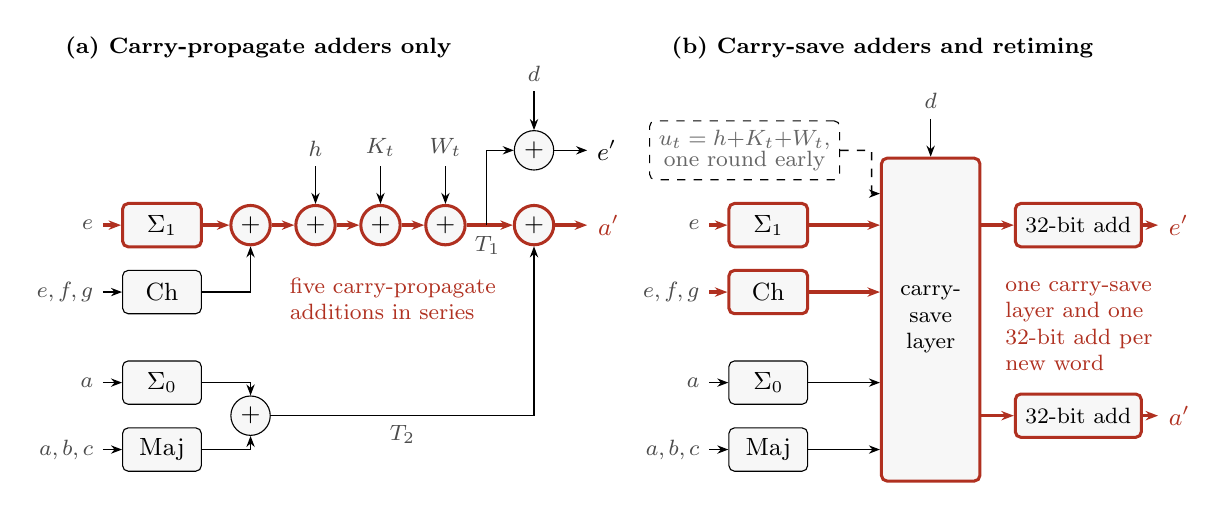
\begin{tikzpicture}[
      x=0.75cm, y=1cm, font=\small,
      fn/.style={draw, rounded corners=2pt, minimum width=1.0cm, minimum height=0.55cm, fill=black!3},
      add/.style={draw, circle, inner sep=0pt, minimum size=0.5cm, fill=black!3},
      csa/.style={draw, rounded corners=2pt, align=center, fill=black!3, font=\footnotesize},
      inp/.style={font=\footnotesize, text=black!70},
      arr/.style={-{Stealth[length=4pt]}, line width=0.5pt},
      hot/.style={-{Stealth[length=4.5pt]}, line width=1.2pt, draw=warn},
      hotbox/.style={draw=warn, line width=1.1pt},
      pre/.style={draw, dashed, rounded corners=2pt, align=center, text=black!60, font=\footnotesize},
      capt/.style={font=\footnotesize\bfseries, anchor=west},
    ]
    % ---------------- (a) textbook datapath ----------------
    \node[capt] at (-1.8,2.25) {(a) Carry-propagate adders only};
    \node[fn, hotbox] (S1) at (0,0) {$\Sigma_1$};
    \node[fn] (Ch) at (0,-0.85) {$\mathrm{Ch}$};
    \node[fn] (S0) at (0,-2.0) {$\Sigma_0$};
    \node[fn] (Mj) at (0,-2.85) {$\mathrm{Maj}$};
    \node[inp, anchor=east] (ie) at (-1.0,0) {$e$};
    \node[inp, anchor=east] at (-1.0,-0.85) {$e,f,g$};
    \node[inp, anchor=east] at (-1.0,-2.0) {$a$};
    \node[inp, anchor=east] at (-1.0,-2.85) {$a,b,c$};
    \draw[hot] (ie) -- (S1);
    \draw[arr] (-1.0,-0.85) -- (Ch);
    \draw[arr] (-1.0,-2.0) -- (S0);
    \draw[arr] (-1.0,-2.85) -- (Mj);
    \node[add, hotbox] (A1) at (1.5,0) {$+$};
    \node[add, hotbox] (A2) at (2.6,0) {$+$};
    \node[add, hotbox] (A3) at (3.7,0) {$+$};
    \node[add, hotbox] (A4) at (4.8,0) {$+$};
    \node[add] (A5) at (1.5,-2.42) {$+$};
    \node[add, hotbox] (A6) at (6.3,0) {$+$};
    \node[add] (A7) at (6.3,0.95) {$+$};
    \draw[hot] (S1) -- (A1);
    \draw[arr] (Ch) -| (A1);
    \draw[hot] (A1) -- (A2);
    \draw[hot] (A2) -- (A3);
    \draw[hot] (A3) -- (A4);
    \draw[arr] (2.6,0.75) node[inp, above] {$h$} -- (A2);
    \draw[arr] (3.7,0.75) node[inp, above] {$K_t$} -- (A3);
    \draw[arr] (4.8,0.75) node[inp, above] {$W_t$} -- (A4);
    \draw[hot] (A4) -- node[inp, below, pos=0.45] {$T_1$} (A6);
    \draw[arr] (5.5,0) |- (A7);
    \draw[arr] (6.3,1.7) node[inp, above] {$d$} -- (A7);
    \draw[arr] (S0) -| (A5);
    \draw[arr] (Mj) -| (A5);
    \draw[arr] (A5) -- node[inp, below, pos=0.5] {$T_2$} (6.3,-2.42) -- (A6);
    \draw[hot] (A6) -- (7.2,0) node[anchor=west, text=warn] {$a'$};
    \draw[arr] (A7) -- (7.2,0.95) node[anchor=west] {$e'$};
    \node[font=\footnotesize, text=warn, align=left, anchor=north west] at (2.0,-0.55)
      {five carry-propagate\\additions in series};

    % ---------------- (b) carry-save + retiming ----------------
    \begin{scope}[xshift=7.7cm]
      \node[capt] at (-1.8,2.25) {(b) Carry-save adders and retiming};
      \node[fn, hotbox] (S1b) at (0,0) {$\Sigma_1$};
      \node[fn, hotbox] (Chb) at (0,-0.85) {$\mathrm{Ch}$};
      \node[fn] (S0b) at (0,-2.0) {$\Sigma_0$};
      \node[fn] (Mjb) at (0,-2.85) {$\mathrm{Maj}$};
      \node[inp, anchor=east] (ieb) at (-1.0,0) {$e$};
      \node[inp, anchor=east] (iefg) at (-1.0,-0.85) {$e,f,g$};
      \node[inp, anchor=east] at (-1.0,-2.0) {$a$};
      \node[inp, anchor=east] at (-1.0,-2.85) {$a,b,c$};
      \draw[hot] (ieb) -- (S1b);
      \draw[hot] (iefg) -- (Chb);
      \draw[arr] (-1.0,-2.0) -- (S0b);
      \draw[arr] (-1.0,-2.85) -- (Mjb);
      \node[pre] (u) at (-0.4,0.95) {$u_t = h{+}K_t{+}W_t$,\\[-2pt]one round early};
      \node[csa, hotbox, minimum width=1.25cm, minimum height=4.1cm] (C) at (2.75,-1.2)
        {carry-\\save\\layer};
      \draw[hot] (S1b) -- (S1b -| C.west);
      \draw[hot] (Chb) -- (Chb -| C.west);
      \draw[arr] (S0b) -- (S0b -| C.west);
      \draw[arr] (Mjb) -- (Mjb -| C.west);
      \draw[arr, dashed] (u.east) -| (1.75,0.4) -- ($(C.west)+(0,1.6)$);
      \draw[arr] (2.75,1.35) node[inp, above] {$d$} -- (C.north);
      \node[csa, hotbox, minimum width=1.6cm, minimum height=0.55cm] (P1) at (5.25,0) {32-bit add};
      \node[csa, hotbox, minimum width=1.6cm, minimum height=0.55cm] (P2) at (5.25,-2.42) {32-bit add};
      \draw[hot] ($(C.east)+(0,1.2)$) -- (P1.west);
      \draw[hot] ($(C.east)+(0,-1.22)$) -- (P2.west);
      \draw[hot] (P1) -- (6.6,0) node[anchor=west, text=warn] {$e'$};
      \draw[hot] (P2) -- (6.6,-2.42) node[anchor=west, text=warn] {$a'$};
      \node[font=\footnotesize, text=warn, align=left, anchor=north west] at (3.85,-0.6)
        {one carry-save\\layer and one\\32-bit add per\\new word};
    \end{scope}
  \end{tikzpicture}
  \caption{One SHA-256 round as a circuit, with the path that limits a chain's latency in red. Inputs on the left are the current state words; $a'$ and $e'$ return to the state registers for the next round. (a)~A direct implementation adds the terms with 32-bit carry-propagate adders, which puts several of them in series. (b)~With carry-save adders and retiming~\cite{LCV07}, $u_t = h + K_t + W_t$ is computed during the previous round, since $h$ is the previous $g$. The remaining terms are reduced to two numbers in a carry-save layer, whose depth does not depend on the word length, and each new word needs one carry-propagate addition. The drawing is schematic; the retimed datapath of~\cite{LCV07} differs in detail.}
  \label{fig:sha-round}
\end{figure}


A chain step $F_i$ hashes 52 bytes, so it is one compression. The message words $W_t$ depend only on the step's input and can be computed alongside the rounds, so the latency of a step is that of the 64 rounds.

\paragraph{How SHA-256 is computed in hardware.}
Assumption A2 can be examined against the structure of SHA-256. One SHA-256 compression is 64 rounds, and each round needs the exact output of the previous one. The new state words are sums of up to five 32-bit terms. Some of them, such as the round constant and the message word, can be added ahead of time, but the next round applies rotations and bitwise functions to the exact bits of the result. Every round must therefore finish at least one 32-bit addition with full carry propagation, plus a few levels of logic. Lee, Chan and Verbauwhede~\cite{LCV07} show that this much is also enough: with carry-save adders and retiming, the loop through one round needs one carry-propagate addition, one carry-save layer and the choice function $\mathrm{Ch}$. \Cref{fig:sha-round} shows both datapaths.

Pipelining raises throughput but not the latency of one chain, since each step starts from the previous step's output. Unrolling removes the registers between rounds, so the relevant floor is the one for logic alone. Hence $\ell$ is roughly 64 times the shortest critical path of one round, measured over many unrolled rounds.

\paragraph{The circuit model.}
The model row of \cref{tab:pricing} quantifies this argument. Its unit is the FO4, the delay of an inverter driving four copies of itself. It estimates the round loop of Lee et al.\ at 10--17 FO4: 7--12 for a fast 32-bit adder~\cite{HS03} and 3--5 that we assume for the carry-save layer and $\mathrm{Ch}$. Predicted FO4 delays for 3--5\,nm processes are 4.3--4.7\,ps~\cite{NCTI21}. Then 64 rounds take
\[
  64 \times 10 \times 4.3\,\text{ps} = 2.75\,\text{ns}
  \quad\text{to}\quad
  64 \times 17 \times 4.7\,\text{ps} = 5.11\,\text{ns},
\]
and with 0.1--0.3\,ns for the final addition and startup, 2.85--5.41\,ns. Our allowance of 1 to 1.8 times for wires, cell choice and registers gives 2.9--9.7\,ns, that is, $A \approx 1.3$--$4.5$.

As a cross-check, Intel's mining patent describes a state update 13 logic levels deep~\cite{SSM18}; if each level cost one FO4, which is optimistic, a hash would take 3.6--3.9\,ns. A process shrink by itself gives only $A \approx 1.3$. At 3.5\,ns a round has 55\,ps, about 12 FO4, so the design point needs a highly optimized custom datapath and sits near the aggressive end of the model. The model's lower end is a conditional estimate, not a physical bound, and no published design that we know of comes close to it.

\paragraph{Mining hardware.}
Bitcoin mining chips are the SHA-256 circuits built in the largest numbers, but they are designed for energy per hash, not latency. Intel's Bonanza Mine~\cite{SKR+22} has 258 fully unrolled double-SHA-256 engines on a 7\,nm die. It runs at 355\,mV and 1.35--1.6\,GHz and computes 137 billion hashes per second at 55\,J per terahash. TICA~\cite{LHZ+22} pipelines the 64 rounds into 64 stages at 0.3\,V in 28\,nm. Both lower the supply voltage close to the threshold, where gates are several times slower, and recover throughput with many engines. Neither reports the latency of one hash. If each cycle of Bonanza Mine advanced one round, one compression would take 40--47\,ns, ten times our 3.5\,ns. A chain attacker would build the opposite: one engine at high voltage, with no registers between rounds.

\paragraph{The precedent of verifiable delay functions.}
Work on verifiable delay functions faced the same question and also answered it with a stated factor: Drake proposed $A_{\max} = 10$ as a conservative parameter for RSA-based VDFs, hoping that public ASICs would bring it to about 5~\cite{Drake18}. Here $A = 10$ means $\ell = 1.3$\,ns, about 4.5 FO4 per round, outside the model but not ruled out. \Cref{sec:open} lists a careful estimate as the most important open question.


\end{document}
